\chapter{Grammar}
\label{ch:grammar}

The fact that corpora are most easily accessed via words (or word forms) is also reflected in many corpus studies focusing on various aspects of grammatical structure. Many such studies either take (sets of) words as a starting point for studying various aspects of grammatical structure, or they take easily identifiable aspects of grammatical structure as a starting point for studying the distribution of words. However, as the case studies of the English possessive constructions in Chapter \ref{ch:quantifyingresearch} and Chapter \ref{ch:significancetesting} showed, grammatical structures can be (and are) also studied in their own right, for example with respect to semantic, information-structural and other restrictions they place on particular slots or sequences of slots, or with their distribution across texts, text types, demographic groups or varieties.

\section{Grammar in corpora}
\label{sec:grammarincorpora}

There are two major problems to be solved when searching corpora for grammatical structures. We discussed both of them to some extent in Chapter \ref{ch:retrievalannotation}, but let us briefly recapitulate and elaborate some aspects of the discussion before turning to the case studies.

First, we must operationally define the structure itself in such a way that we (and other researchers) can reliably categorize potential instances as manifesting the structure or not. This may be relatively straightforward in the case of simple grammatical structures that can be characterized based on tangible and stable characteristics, such as particular configurations of grammatical morphemes and/or categories occurring in sequences that reflect hierarchical relationships relatively directly. It becomes difficult, if not impossible, with complex structures, especially in frameworks that characterize such structures with recourse to abstract, non-tangible and theory-dependent constructs (see \citet{sampson_english_1995} for an attempt at a comprehensive annotation scheme for the grammar of English).

Second, we must define a query that will allow us to retrieve potential candidates from our corpus in the first place (a problem we discussed in some detail in Chapter \ref{ch:retrievalannotation}). Again, this is simpler in the case of morphologically marked and relatively simple grammatical structures or example, the \textit{s}-possessive (as defined above) is typically characterized by the sequence $\langle$ \texttt{[pos="noun"] [word="'s"\%c] [pos="adjective"]* [pos="noun"]} $\rangle$ in corpora containing texts in standard orthography; it can thus be retrieved from a POS-tagged corpus with a fairly high degree of precision and recall. However, even this simple case is more complex than it seems. The query will produce false hits, as in the sequence just given, \textit{'s} it may also stand for the verb \textit{be} (\textit{Sam's head of marketing}); and it will produce false misses, as the modified nominal may not always be directly adjacent to the \textit{'s} (for example in \textit{This office is Sam's} or in \textit{Sam's friends and family}) and the \textit{s}-possessive may be represented by an apostrophe alone (for example in \textit{his friends' families}).

Other structures may be difficult to retrieve even though they can be characterized straightforwardly: most linguists would agree, for example, that transitive verbs, are verbs that take a direct object. However, this is of very little help in retrieving transitive verbs even from a POS-tagged corpus, since many noun-phrases following a verb will not be direct objects (\textit{Sam slept the whole day}) and direct objects do not necessarily follow their verb (\textit{Sam, I have not seen}); in addition, noun phrases themselves are not trivial to retrieve.

Yet other structures may be easy to retrieve, but not without retrieving many false hits at the same time. This is the case with ambiguous structures like the \textit{of}-possessive, which can be retrieved by a query along the lines of $\langle$ \texttt{[pos="noun"] [pos="determiner"]? [pos="adjective"]* [pos="noun"]} $\rangle$, which will also retrieve, among other things, partitive and quantitative uses of the \textit{of}\hyp{}construction).

Finally, structures characterized with reference to invisible theoretical constructs are so difficult to retrieve that this, in itself, may be a good reason to avoid such invisible constructs whenever possible when characterizing linguistic phenomena that we plan to investigate empirically.

These difficulties do not keep corpus linguists from investigating grammatical structures, even very abstract ones, retrieving the relevant data by mind\hyp{}numb\-ing and time\hyp{}consuming manual analysis of the results of very broad searches or even of the corpus itself, if necessary. But it is probably one reason why so much grammatical research in corpus linguistics takes a word-centered approach.

A second reason is that it allows us to transfer well-established collocational methods to the study of grammar. In the preceding chapter we saw that while collocation research often takes a sequential approach to co-occurrence, counting as potential collocates of a node word any word within a given span around it, it is not uncommon to see a structure-sensitive approach that considers only those potential collocates that occur in a particular grammatical position relative to each other (for example, adjectives relative to the nouns they modify or vice versa). In this approach, grammatical structure is already present in the design, even though it remains in the background. We can move these types of grammatical structure into the focus of our investigation, giving us a range of research designs where one variable consists of (part of) the lexicon (with values that are individual words) and one variable consists of some aspect of grammatical structure. In these studies, the retrieval becomes somewhat less of a problem, as we can search for lexical items and identify the grammatical structures in our search results afterwards, though identifying these structures reliably remains non-trivial. We will begin with word-centered case studies and then move towards more genuinely grammatical research designs.

\section{Case studies}
\label{sec:grammarcasestudies}

\subsection{Collocational frameworks and grammar patterns}
\label{sec:collocationalframeworksandgrammarpatterns}

An early extension of collocation research to the association between words and grammatical structure is \citet{renouf_collocational_1991}. The authors introduce a novel construct, the \textit{collocational framework}, which they define as ``a discontinuous sequence of two words, positioned at one word remove from each other'', where the two words in question are always function words -- examples are [\textit{a} \_\_ \textit{of}], [\textit{an} \_\_ \textit{of}], [\textit{too} \_\_ \textit{to}] or [\textit{many} \_\_ \textit{of}] (note that \textit{a} and \textit{an} are treated as constituents of different frameworks, showing a radically word-form-oriented approach to grammar). Renouf and Sinclair are particularly interested in classes of items that fill the position in the middle of collocational frameworks and they see the fact that these items tend to form semantically coherent classes as evidence that collocational frameworks are relevant items of linguistic structure.

The idea behind collocational frameworks was subsequently extended by \citet{hunston_pattern_2000} to more canonical linguistic structures, ranging from very general valency patterns (such as [V NP] or [V NP NP]) to very specific structures like [\textit{there} + Linking Verb + \textit{something} Adjective + \textit{about} NP] (as in \textit{There was something masculine about the dark wood dining room} \citet[51, 53, 106]{hunston_pattern_2000}). Their essential insight is similar to Renouf and Sinclair's: that such structures (which they call ``grammar patterns''), are meaningful and that their meaning is manifest in the collocates in central slots::

\begin{quotation}
The patterns of a word can be defined as all the words and structures which are regularly associated with the word and which contribute to its meaning. A pattern can be identified if a combination of words occurs relatively frequently, if it is dependent on a particular word choice, and if there is a clear meaning associated with it \citep[37]{hunston_pattern_2000}.
\end{quotation}

Collocational frameworks and especially grammar patterns have an immediate applied relevance: the COBUILD dictionaries included the most frequently found patterns for each word in their entries from 1995 onward and there is a two-volume descriptive grammar of the patterns of verbs \citep{francis_collins_1996} and nouns and adjectives \citep{francis_collins_1998}; there were also attempts to identify grammar patterns automatically \citep[cf.][]{mason_automatic_2004}. Research on collocational frameworks and grammar patterns is mainly descriptive and takes place in applied contexts, but \citet{hunston_pattern_2000} argue very explicitly for a usage-based theory of grammar on the basis of their descriptions (note that the definition quoted above is strongly reminiscent of the way constructions were later defined in Construction Grammar \citep[4]{goldberg_constructions:_1995}, a point I will return to in the Epilogue of this book.

\subsubsection{Case study: [\textit{a} \_\_ \textit{of}]}
\label{sec:anof}

As an example of a collocational framework, consider [\textit{a} \_\_ \textit{of}], one of the patterns that \citet{renouf_collocational_1991} use to introduce their construct. Renouf and Sinclair use an early version of the \textit{Birmingham Collection of English Text}, which is no longer accessible. To enable us to look at the methodological issues raised by collocational frameworks more closely, I have therefore replicated their study using the BNC. As far as is possible to tell from the data presented in \citet{renouf_collocational_1991}, they simply extracted all words occurring in the framework, without paying attention to part-of-speech tagging, so I did the same; it is unclear whether their query was case-sensitive, I used a case insensitive query for the BNC data).

Table \ref{tab:axoftwocorpora} shows the data from \citet{renouf_collocational_1991} and from the BNC. As you can see, the results are roughly comparable, but differ noticeably in some details -- two corpora will never give you quite the same result even with general patterns like the one under investigation.

\begin{table}[!htbp]
\caption{The collocational framework  [\textit{a} \_\_ \textit{of}] in two corpora}
\label{tab:axoftwocorpora}
\resizebox{\textwidth}{!}{%
\begin{tabular}[t]{lS|lS||lS|lS}
\lsptoprule
\multicolumn{4}{c||}{\makecell[tc]{Birmingham Collection of English Text}} & \multicolumn{4}{c}{\makecell[tc]{British National Corpus}} \\
\midrule
\multicolumn{2}{c}{\makecell[tc]{(a)}} & \multicolumn{2}{c||}{\makecell[tc]{(b)}} & \multicolumn{2}{c}{\makecell[tc]{(a)}} & \multicolumn{2}{c}{\makecell[tc]{(b)}} \\
\multicolumn{1}{l}{\makecell[tl]{Collocate}} & \multicolumn{1}{l|}{\makecell[tl]{Frequency}} & \multicolumn{1}{l}{\makecell[tl]{Collocate}} & \multicolumn{1}{l||}{\makecell[tl]{Percent}} & \multicolumn{1}{l}{\makecell[tl]{Collocate}} & \multicolumn{1}{l|}{\makecell[tl]{Frequency}} & \multicolumn{1}{l}{\makecell[tl]{Collocate}} & \multicolumn{1}{l}{\makecell[tl]{Percent}} \\
\midrule
\textit{lot} & 1322 & \textit{couple} & 62 & \textit{number} & 13766 & \textit{couple} & 55.72 \\
\textit{kind} & 864 & \textit{series} & 57 & \textit{lot} & 13649 & \textit{lot} & 48.81 \\
\textit{number} & 762 & \textit{pair} & 54 & \textit{couple} & 6620 & \textit{variety} & 47.54 \\
\textit{couple} & 685 & \textit{lot} & 53 & \textit{series} & 5655 & \textit{series} & 39.76 \\
\textit{matter} & 550 & \textit{piece} & 36 & \textit{result} & 5596 & \textit{pair} & 36.63 \\
\textit{sort} & 451 & \textit{quarter} & 36 & \textit{bit} & 4879 & \textit{number} & 28.21 \\
\textit{series} & 438 & \textit{variety} & 35 & \textit{matter} & 4561 & \textit{piece} & 26.96 \\
\textit{piece} & 414 & \textit{member} & 34 & \textit{variety} & 4113 & \textit{result} & 25.54 \\
\textit{bit} & 379 & \textit{number} & 30 & \textit{member} & 3650 & \textit{member} & 21.00 \\
\textit{sense} & 356 & \textit{kind} & 21 & \textit{range} & 3193 & \textit{matter} & 20.97 \\
\textit{pair} & 320 & \textit{sort} & 21 & \textit{group} & 3081 & \textit{bit} & 18.43 \\
\textit{member} & 302 & \textit{matter} & 20 & \textit{kind} & 2522 & \textit{range} & 15.76 \\
\textit{group} & 293 & \textit{result} & 20 & \textit{piece} & 2430 & \textit{list} & 14.22 \\
\textit{result} & 268 & \textit{bit} & 19 & \textit{sense} & 2398 & \textit{sense} & 11.23 \\
\textit{part} & 222 & \textit{bottle} & 17 & \textit{period} & 2350 & \textit{kind} & 10.71 \\
\textit{variety} & 216 & \textit{sense} & 13 & \textit{set} & 2253 & \textit{period} & 9.75 \\
\textit{state} & 205 & \textit{group} & 11 & \textit{sort} & 2243 & \textit{sort} & 8.33 \\
\textit{bottle} & 175 & \textit{state} & 7 & \textit{pair} & 2170 & \textit{group} & 7.49 \\
\textit{man} & 174 & \textit{part} & 5 & \textit{way} & 1942 & \textit{set} & 5.10 \\
\textit{quarter} & 174 & \textit{man} & 2 & \textit{list} & 1770 & \textit{way} & 2.03 \\
\lspbottomrule
\end{tabular}}
\end{table}
% query: BNC; [word="a"%c] [] [word="of"%c]; count A by word%c

Renouf and Sinclair first present the twenty items occurring most frequently in the collocational framework, shown in the columns labeled (a). These are, roughly speaking, the words most typical for the collocational framework: when we encounter the framework (in a corpus or in real life), these are the words that are most probable to fill the slot between \textit{a} and \textit{of}. Renouf and Sinclair then point out that the frequency of these items in the collocational framework does not correspond to their frequency in the corpus as a whole, where, for example, \textit{man} is the most frequent of their twenty words, and \textit{lot} is only the ninth-most frequent. The ``promotion of \textit{lot} to the top of the list'' in the framework [\textit{a} \_\_ \textit{of}], they argue, shows that it is its ``tightest collocation''. As discussed in Chapter \ref{ch:collocation}, association measures are the best way to asses the difference in frequency of an item under a specific condition (here, the presence of the collocational framework) from its general frequency and I will present the strongest collocates as determined by the $G^2$ statistic below.

Renouf and Sinclair choose a different strategy: they calculate for each item, what percentage of all occurrences of that item is within the collocational framework. The results are shown in the columns labeled (b) (for example, \textit{number} occurrs in the BNC a total of \num{48806} times, so the \num{13799} times that it occurs in the pattern [\textit{a} \_\_ \textit{of}] account for \num{28.21} percent of its occurrences). As you can see, the order changes slightly, but the basic result appears to remain the same. Broadly speaking, the most strongly associated words in both corpora and by either measure tend to be related to quantities (e.g. \textit{lot}, \textit{number}, \textit{couple}), part-whole relations (e.g. \textit{piece}, \textit{member}, \textit{group}, \textit{part}), or types (e.g. \textit{sort} or \textit{variety}. This kind of semantic coherence is presented by Renouf and Sinclair as evidence that collocational frameworks are relevant units of language.

Keeping this in mind, let us discuss the difference between frequency and percentages in some more detail. Note, first, that the reason the results do not change perceptibly is because Renouf and Sinclair do not determine the percentage of occurrences of words inside [\textit{a} \_\_ \textit{of}] for all words in the framework, but only for the twenty nouns that they have already identified as most frequent -- the columns labeled (b) thus represent a ranking based on a mixed strategy of preselecting words by their raw frequency and then ranking them by their proportions inside and outside the framework. 

If we were to omit the pre-selection stage and calculate the percentages for all words occurring in the framework, as we should, if these percentages are relevant, we would find 477 words in the BNC that occur exclusively in the framework, and thus all have an association strength of 100 percent -- among them words that fit the proposed semantic preferences of the pattern, like \textit{barrelful}, words that do not fit, like \textit{bomb-burst}, \textit{hyserisation} or \textit{Jesuitism}, and many misspellings, like \textit{fct} (for \textit{fact}) and \textit{numbe} and \textit{numbr} (for \textit{number}). The problem here is that percentages, like some other association measures, massively overestimate the importance of rare events. In order to increase the quality of the results, let us remove all words that occur five times or less in the BNC. The twenty words in Table \ref{tab:axofpercent} are then the words with the highest percentages of occurrence in the framework [\textit{a} \_\_ \textit{of}].

\begin{table}[!htbp]
\caption{The collocational framework  [\textit{a} \_\_ \textit{of}] in the BNC by percentage of occurrences}
\label{tab:axofpercent}
\resizebox{.6\textwidth}{!}{%
\begin{tabular}[t]{lSSS}
\lsptoprule
\multicolumn{1}{l}{\makecell[tl]{Collocate}} & \multicolumn{1}{l}{\makecell[tl]{n(Framework)}} & \multicolumn{1}{l}{\makecell[tl]{n(Corpus)}} & \multicolumn{1}{l}{\makecell[tl]{Percent}} \\
\midrule
\textit{headful} & 6 & 6 & 1 \\
\textit{roomful} & 19 & 22 & 0.863636363636364 \\
\textit{modicum} & 61 & 73 & 0.835616438356164 \\
\textit{fistful} & 45 & 57 & 0.789473684210526 \\
\textit{figment} & 48 & 62 & 0.774193548387097 \\
\textit{foretaste} & 48 & 64 & 0.75 \\
\textit{pocketful} & 9 & 12 & 0.75 \\
\textit{smattering} & 43 & 60 & 0.716666666666667 \\
\textit{houseful} & 10 & 14 & 0.714285714285714 \\
\textit{gaggle} & 35 & 49 & 0.714285714285714 \\
\textit{founder-member} & 17 & 24 & 0.708333333333333 \\
\textit{hatful} & 9 & 13 & 0.692307692307692 \\
\textit{handful} & 917 & 1342 & 0.683308494783905 \\
\textit{coming-together} & 5 & 8 & 0.625 \\
\textit{smidgeon} & 5 & 8 & 0.625 \\
\textit{multitude} & 288 & 467 & 0.616702355460385 \\
\textit{superset} & 8 & 13 & 0.615384615384615 \\
\textit{lungful} & 8 & 13 & 0.615384615384615 \\
\textit{bevy} & 22 & 36 & 0.611111111111111 \\
\textit{surfeit} & 32 & 53 & 0.60377358490566 \\
\lspbottomrule
\end{tabular}}
\end{table}

This list is obviously completely different from the one in \citet{renouf_collocational_1991} or our replication. We would not want to call them typical for [\textit{a} \_\_ \textit{of}], in the sense that it is not very probable that we will encounter them in this collocational framework. However, note that they generally represent the same categories as the words in Table \ref{tab:axoftwocorpora}, namely ``quantity'' and ``part-whole'', indicating a relevant relation to the framework. This relation is, in fact, the counterpart to the one shown in Table \ref{tab:axoftwocorpora}: These are words for which the framework [\textit{a} \_\_ \textit{of}] is typical, in the sense that if we encounter these words, it is very probable that they will be accompanied by this collocational framework.

There are words that are typical for a particular framework, and there are frameworks that are typical for particular words; this difference in perspective may be of interest in particular research designs \citep[cf.][]{stefanowitsch_corpus-based_2016} for further discussion. Generally, however, it is best to use an established association measure that will not overestimate rare events. Table \ref{tab:axofcollframe} shows the fifteen most strongly associated word in the framework based on the $G^2$ statistic.

\begin{table}[!htbp]
\caption{Top collocates of the collocational framework [\textit{a} \_\_ \textit{of}] (BNC)}
\label{tab:axofcollframe}
\resizebox{\textwidth}{!}{%
\begin{tabular}[t]{l *{4}{S[table-format=5]} S}
\lsptoprule
\multicolumn{1}{c}{\makecell[tc]{\textvv{Collexeme}}} &
	\multicolumn{1}{c}{\makecell[tc]{Collocate in \\ Framework}} & 
	\multicolumn{1}{c}{\makecell[tc]{Collocate outside \\ Framework}} & 
	\multicolumn{1}{c}{\makecell[tc]{Other verbs \\ in Framework}} & 
	\multicolumn{1}{c}{\makecell[tc]{Other verbs \\ outside Framework}} & 
	\multicolumn{1}{c}{\makecell[tc]{G\textsuperscript{2}}} \\
\midrule
\textit{lot} & 13649 & 13570 & 231601 & 98104963 & 126731.193490679 \\
\textit{number} & 13766 & 33607 & 231484 & 98084926 & 108873.769031002 \\
\textit{couple} & 6620 & 5065 & 238630 & 98113468 & 63575.7283209112 \\
\textit{series} & 5655 & 7658 & 239595 & 98110875 & 49809.0439876969 \\
\textit{result} & 5596 & 16206 & 239654 & 98102327 & 42459.3430147308 \\
\textit{variety} & 4113 & 4322 & 241137 & 98114211 & 37710.0753786109 \\
\textit{bit} & 4879 & 21110 & 240371 & 98097423 & 33590.5137196649 \\
\textit{matter} & 4561 & 17062 & 240689 & 98101471 & 32567.4848172841 \\
\textit{member} & 3650 & 10143 & 241600 & 98108390 & 27921.3175208155 \\
\textit{range} & 3193 & 16499 & 242057 & 98102034 & 20946.0966509352 \\
\textit{piece} & 2430 & 6486 & 242820 & 98112047 & 18742.2336813293 \\
\textit{pair} & 2170 & 3682 & 243080 & 98114851 & 18334.5738533205 \\
\textit{group} & 3081 & 30068 & 242169 & 98088465 & 16617.232995328 \\
\textit{kind} & 2522 & 20848 & 242728 & 98097685 & 14372.037145012 \\
\textit{sense} & 2398 & 18815 & 242852 & 98099718 & 13895.1731660216 \\
\lspbottomrule
\end{tabular}}
\end{table}

This case study has introduced the notion of collocational frameworks as a simple way of studying the relationship between words and their grammatical context and the potential functional nature of this relationship. It is also meant as a reminder of the different results that different corpora and especially different measures of collocation strength will yield different results.

\subsubsection{Case study: [\textit{there} V\textsubscript{link} \textit{something} ADJ \textit{about} NP]}
\label{sec:itbeadto}

As an example of a grammar pattern, consider [\textit{there} V\textsubscript{link} \textit{something} ADJ \textit{about} NP] \citep[105--106]{hunston_pattern_2000}. As is typical of grammar patterns, this pattern constitutes a canonical unit of grammatical structure -- unlike Renouf and Sinclair's collocational frameworks.

Hunston and Francis mention this pattern only in passing, noting that it ``has the function of evaluating the person or thing indicated in the noun group following \textit{about}''. Their usual procedure (which they skip in this case) is to back up such observations concerning the meaning of grammar patterns by listing the most frequent items occurring in this pattern and showing that these form one or more semantic classes (similar to the procedure used by Renouf and Sinclair). In (\ref{ex:sthadjaboutgrampat}), I list all words occurring in the British National Corpus more than twice, with their frequency in parentheses:

\begin{exe}
\ex \textit{odd} (21), \textit{special} (20), \textit{different} (18), \textit{familiar} (16), \textit{strange} (13), \textit{sinister} (8), \textit{disturbing} (5), \textit{funny} (5), \textit{wrong} (5), \textit{absurd} (4), \textit{appealing} (4), \textit{attractive} (4), \textit{fishy} (4), \textit{paradoxical} (4), \textit{sad} (4), \textit{unusual} (4), \textit{impressive} (3), \textit{shocking} (3), \textit{spooky} (3), \textit{touching} (3), \textit{unique} (3), \textit{unsatisfactory} (3)
\label{ex:sthadjaboutgrampat}
\end{exe}

The list clearly supports Hunston and Francis's claim about the meaning of this grammar pattern -- most of the adjectives are inherently evaluative. There are a few exceptions -- \textit{different}, \textit{special}, \textit{unusual} and \textit{unique} do not have to be used evaluatively. If they occur in the pattern [\textit{there} V\textsubscript{link} \textit{something} ADJ \textit{about} NP], however, they are likely to be interpreted evaluatively.

As \citet[105]{hunston_pattern_2000} point out: ``Even when potentially neutral words such as nationality words, or words such as \textit{masculine} and \textit{feminine}, are used in this pattern, they take on an evaluative meaning. This is, in fact, a crucial feature of grammar patterns, as it demonstrates that these patterns themselves are meaningful and are able to impart their meaning on words occurring in them. The following examples demonstrate this:

\begin{exe}
\ex
\begin{xlist} 
\label{ex:sthadjaboutcoercion}
\ex There is something horribly cyclical about television advertising. (BNC CBC)
\ex It is a big, square box, painted dirty white, and, although he is always knocking through, extending, repapering and spring-cleaning, there is something dead about the place. (BNC HR9)
\ex At least it didn't sound now quite like a typewriter, but there was something metallic about it. (BNC J54)
\end{xlist}
\end{exe}

The adjective \textit{cyclical} is neutral, but the adverb \textit{horribly} shows that it is meant evaluatively in (\ref{ex:sthadjaboutcoercion}a); \textit{dead} in its literal sense is purely descriptive, but when applied to things (like a house in (\ref{ex:sthadjaboutcoercion}b)), it becomes an evaluation; finally, \textit{metallic} is also neutral, but it is used to evaluate a sound negatively in (\ref{ex:sthadjaboutcoercion}c), as shown by the phrasing \textit{at least ... but}.

Instead of listing frequencies, of course, we could calculate the association strenght between the pattern [\textit{there} V\textsubscript{link} \textit{something} ADJ \textit{about} NP] and the adjectives occurring in it. I will discuss in more detail how this is done in the next subsection; for now, suffice it to say that it would give us the ranking in Table \ref{tab:sthadjaboutcollex}.

\begin{table}[!htbp]
\caption{Most strongly associated adjectives in the pattern [\textit{there} V\textsubscript{link} \textit{something} ADJ \textit{about} NP]}
\label{tab:sthadjaboutcollex}
\resizebox{\textwidth}{!}{%
\begin{tabular}[t]{l *{4}{S[table-format=5]} S}
\lsptoprule
\multicolumn{1}{c}{\makecell[tc]{\textvv{Collocate}}} &
	\multicolumn{1}{c}{\makecell[tc]{Frequency in \\ the pattern}} & 
	\multicolumn{1}{c}{\makecell[tc]{Frequency outside \\ the pattern}} & 
	\multicolumn{1}{c}{\makecell[tc]{Other words \\ in the pattern}} & 
	\multicolumn{1}{c}{\makecell[tc]{Other words \\ outside the pattern}} & 
	\multicolumn{1}{c}{\makecell[tc]{G\textsuperscript{2}}} \\
\midrule
\textit{odd} & 21 & 4277 & 317 & 7854379 & 158.555586224863 \\
\textit{familiar} & 16 & 5503 & 322 & 7853153 & 104.011464887408 \\
\textit{special} & 20 & 21725 & 318 & 7836931 & 85.4950969420225 \\
\textit{strange} & 13 & 6026 & 325 & 7852630 & 76.7731710162547 \\
\textit{sinister} & 8 & 661 & 330 & 7857995 & 74.3869080936388 \\
\textit{different} & 18 & 47503 & 320 & 7811153 & 47.1835415212247 \\
\textit{fishy} & 4 & 104 & 334 & 7858552 & 46.2726661691692 \\
\textit{paradoxical} & 4 & 258 & 334 & 7858398 & 39.1074203555728 \\
\textit{disturbing} & 5 & 1037 & 333 & 7857619 & 37.3328860586622 \\
\textit{spooky} & 3 & 128 & 335 & 7858528 & 31.772080110119 \\
\textit{absurd} & 4 & 922 & 334 & 7857734 & 29.0195484212928 \\
\textit{appealing} & 4 & 976 & 334 & 7857680 & 28.5697575205141 \\
\textit{funny} & 5 & 4301 & 333 & 7854355 & 23.4026921680739 \\
\textit{shocking} & 3 & 541 & 335 & 7858115 & 23.2121219613433 \\
\textit{touching} & 3 & 613 & 335 & 7858043 & 22.4705339888496 \\
\textit{creepy} & 2 & 63 & 336 & 7858593 & 22.3709565523057 \\
\textit{unsatisfactory} & 3 & 757 & 335 & 7857899 & 21.2196064379622 \\
\textit{shifty} & 2 & 97 & 336 & 7858559 & 20.6694329526023 \\
\textit{uncatlike} & 1 & 0 & 337 & 7858656 & 20.1112079152458 \\
\lspbottomrule
\end{tabular}}
\end{table}

The ranking does not differ radically from the ranking by frequency in (\ref{ex:sthadjaboutcoercion}) above, but note that the descriptive adjectives \textit{special} and \textit{different} are moved down the list a few ranks and \textit{unique} and \textit{unusual} disappear from the top twenty, sharpening the semantic profile of the pattern.

This case study is meant to introduce the notion of grammar patterns and to show that these patterns often have a relatively stable meaning that can be uncovered by looking at the words that are frequent in (or strongly associated with) them. Like the preceding case study, it also introduced the idea that the relationship between words and units of grammatical structure can be investigated using the logic of association measures. The next sections look at this in more detail.

\subsection{Collostructional analysis}
\label{sec:collostructionalanalysis}

Under the definition of corpus linguistics used throughout this book, there should be nothing surprising about the idea of investigating the relationship between words and units of grammatical structure based on association measures: a grammatical structure is just another condition under which we can observe the occurrence of lexical items. This is the basic idea of ``collostructional analysis'', a methodological perspective first proposed in \citet{stefanowitsch_collostructions:_2003}. This perspective builds on ideas in collocation analysis, colligation analysis (cf. Section \ref{sec:grammarandcontext} below) and pattern grammar, but is more rigorously quantitative empirically, and grounded in construction grammar conceptually. It has been applied in all areas of grammar, with a focus on argument structur (see \citet{ludeling_corpora_2009} and \citet{hoffmann_collostructional_2013} for overviews). Like collocation analysis, it is generally inductive, but it can also be used to test certain general hypotheses about the meaning of grammatical constructions.

\subsubsection{Case study: The ditransitive}
\label{sec:theditransitive}

\citet{stefanowitsch_collostructions:_2003} investigate, among other things, which verbs are strongly associated with the ditransitive construction (or ditransitive subcategorization, if you don't like constructions). This is a very direct application of the basic research design for collocates introduced in the preceding chapter.

Their design is broadly deductive, as their hypothesis is that constructions have meaning and specifically, that the ditransitive has a ``transfer'' meaning. The design has two nominal variables: \textsc{Argument Structure} (with the \textsc{values} ditransitive and \textsc{other}) and V\textsc{erb} (with values corresponding to all verbs occurring in the construction). The prediction is that the most strongly associated verbs will be verbs of literal or metaphorical transfer. Table \ref{tab:giveditransitive} gives the information needed to calculate the association strength for give (although the procedure should be familiar by now), and Table \ref{tab:verbsditransitive} shows the ten most strongly associated verbs.\footnote{Unlike in the rest of the book, I have to use data from a corpus that is not generally accessible -- the British Component of the International Corpus of English. The reason is that analyses like the ones presented here require a treebank (see Section \ref{sec:annotations} in Chapter \ref{ch:retrievalannotation}), and there is no sufficiently large and generally accessible treebank.}

\begin{table}[!htbp]
\caption{\textit{Give} and the ditransitive (ICE-GB)}
\label{tab:giveditransitive}
\begin{tabular}[t]{llccr}
\lsptoprule
 & & \multicolumn{2}{c}{\textvv{Argument Structure}} & \\
 & & \textvv{ditransitive} & \textvv{$\neg$ditransitive} & Total \\
\midrule
\textvv{\makecell[lt]{Verb}}
	& \textvv{give} 
		& \makecell[t]{\num{461}\\\small{(\num{8.63})}}
		& \makecell[t]{\num{574}\\\small{(\num{1026.37})}}
		& \makecell[t]{\num{1035}\\} \\
	& \textvv{$\neg$give}
		& \makecell[t]{\num{687}\\\small{(\num{1139.37})}}
		& \makecell[t]{\num{135907}\\\small{(\num{135454.63})}}
		& \makecell[t]{\num{136594}\\} \\
\midrule
	& Total
		& \makecell[t]{\num{1148}}
		& \makecell[t]{\num{136481}}
		& \makecell[t]{\num{137629}} \\
\lspbottomrule
\end{tabular}
\end{table}
% chisq.test(matrix(c(461,687,574,135907),ncol=2),corr=FALSE)

\begin{table}[!htbp]
\caption{The verbs in the ditransitive construction (ICE-GB, \citet[229]{stefanowitsch_collostructions:_2003})}
\label{tab:verbsditransitive}
\resizebox{\textwidth}{!}{%
\begin{tabular}[t]{l *{4}{S[table-format=5]} r}
\lsptoprule
\multicolumn{1}{c}{\makecell[tc]{\textvv{Collexeme}}} &
	\multicolumn{1}{c}{\makecell[tc]{Collexeme with \\ Ditransitive}} & 
	\multicolumn{1}{c}{\makecell[tc]{Collexeme with \\ other ASCs}} & 
	\multicolumn{1}{c}{\makecell[tc]{Other verbs \\ with Ditransitive}} & 
	\multicolumn{1}{c}{\makecell[tc]{Other verbs \\ with other ASCs}} & 
	\multicolumn{1}{c}{\makecell[tc]{p\textsubscript{exact}}} \\
\midrule
\textit{give} & 461 & 687 & 574 & 136942 & 0 \\
\textit{tell} & 128 & 660 & 907 & 136969 & 1.6e-127 \\
\textit{send} & 64 & 280 & 971 & 137349 & 7.26e-68 \\
\textit{offer} & 43 & 152 & 992 & 137477 & 3.31e-49 \\
\textit{show} & 49 & 578 & 986 & 137051 & 2.23e-33 \\
\textit{cost} & 20 & 82 & 1015 & 137547 & 1.12e-22 \\
\textit{teach} & 15 & 76 & 1020 & 137553 & 4.32e-16 \\
\textit{award} & 7 & 9 & 1028 & 137620 & 1.36e-11 \\
\textit{allow} & 18 & 313 & 1017 & 137316 & 1.12e-10 \\
\textit{lend} & 7 & 24 & 1028 & 137605 & 2.85e-09 \\
\lspbottomrule
\end{tabular}}
\end{table}

The hypothesis is corroborated: the top ten collexemes (and most of the other significant collexemes not shown here) refer to literal or metaphorical transfer.

However, note that on the basis of lists like that in Table \ref{tab:verbsditransitivedative} we cannot reject a null hypothesis along the lines of ``There is no relationship between the ditransitive and the encoding of transfer events'', since we did not test this. All we can say is that we can reject null hypotheses stating that there is no relationship between the ditransitive and each individual verb on the list. In practice, this may amount to the same thing, but if we wanted to reject the more general null hypothesis, we would have to code all verbs in the corpus according to whether they are transfer verbs or not, and the show that transfer verbs are significantly more frequent in the ditransitive construction than in the corpus as a whole.

\subsubsection{Case study: Ditransitive and prepositional dative}
\label{sec:ditransitiveandprepositionaldative}

Collostructional analysis can also be applied in the direct comparison of two grammatical constructions (or other grammatical features), analogous to the ``differential collocate'' design discussed in Chapter \ref{ch:collocation}. For example, \citet{gries_extending_2004} compare verbs in the ditransitive and the so-called \textit{to}-dative -- both constructions express transfer meanings, but it has been claimed that the ditransitive encodes a spatially and temporally more direct transfer than the \textit{to}-dative \citep{thompson_iconicity_1987}. If this is the case, it should be reflected in the verbs most strongly associated to one or the other construction in a direct comparison. Table \ref{tab:giveprepdative} shows the data needed to determine for the verb \textit{give} which of the two constructions it is more strongly attracted to.

\begin{table}[!htbp]
\caption{\textit{Give} in the ditransitive and the prepositional dative (ICE-GB)}
\label{tab:giveprepdative}
\begin{tabular}[t]{llccr}
\lsptoprule
 & & \multicolumn{2}{c}{\textvv{Argument Structure}} & \\
 & & \textvv{ditransitive} & \textvv{$\neg$ditransitive} & Total \\
\midrule
\textvv{\makecell[lt]{Verb}}
	& \textvv{give} 
		& \makecell[t]{\num{461}\\\small{(\num{212.68})}}
		& \makecell[t]{\num{574}\\\small{(\num{822.32})}}
		& \makecell[t]{\num{1035}\\} \\
	& \textvv{$\neg$give}
		& \makecell[t]{\num{146}\\\small{(\num{394.32})}}
		& \makecell[t]{\num{1773}\\\small{(\num{1524.68})}}
		& \makecell[t]{\num{1919}\\} \\
\midrule
	& Total
		& \makecell[t]{\num{607}}
		& \makecell[t]{\num{2347}}
		& \makecell[t]{\num{2954}} \\
\lspbottomrule
\end{tabular}
\end{table}
% chisq.test(matrix(c(461,146,574,1773),ncol=2),corr=FALSE)

\textit{Give} is significantly more frequent than expected in the ditransitive and less frequent than expected in the \textit{to-}dative ($p_exact = 1.84E-120$). It is therefore be said to be a \textit{significant distinctive collexeme} of the ditransitive (again, I will use the term \textit{differential} instead of \textit{distinctive} in the following). Table \ref{tab:verbsditransitivedative} shows the top ten differential collexemes for each construction.

\begin{table}[!htbp]
\caption{Verbs the ditransitive and the prepositional dative (ICE-GB, \citet[106]{gries_extending_2004}).}
\label{tab:verbsditransitivedative}
\resizebox{\textwidth}{!}{%
\begin{tabular}[t]{l *{4}{S[table-format=5]} r}
\lsptoprule
\multicolumn{1}{c}{\makecell[tc]{\textvv{Collexeme}}} &
	\multicolumn{1}{c}{\makecell[tc]{Collexeme with \\ Ditransitive}} & 
	\multicolumn{1}{c}{\makecell[tc]{Collexeme with \\ \textit{to}-Dative}} & 
	\multicolumn{1}{c}{\makecell[tc]{Other verbs \\ with Ditransitive}} & 
	\multicolumn{1}{c}{\makecell[tc]{Other verbs \\ with \textit{to}-Dative}} & 
	\multicolumn{1}{c}{\makecell[tc]{p\textsubscript{exact}}} \\
\midrule
\multicolumn{6}{l}{most strongly associated with the ditransitive} \\
\midrule
\textit{give} & 461 & 146 & 574 & 1773 & 1.84E-120 \\
\textit{tell} & 128 & 2 & 907 & 1917 & 8.77E-58 \\
\textit{show} & 49 & 15 & 986 & 1904 & 8.32E-12 \\
\textit{offer} & 43 & 15 & 992 & 1904 & 9.95E-10 \\
\textit{cost} & 20 & 1 & 1015 & 1918 & 9.71E-09 \\
\textit{teach} & 15 & 1 & 1020 & 1918 & 1.49E-06 \\
\textit{wish} & 9 & 1 & 1026 & 1918 & 0.0005 \\
\textit{ask} & 12 & 4 & 1023 & 1915 & 0.0013 \\
\textit{promise} & 7 & 1 & 1028 & 1918 & 0.0036 \\
\textit{deny} & 8 & 3 & 1027 & 1916 & 0.0122 \\
\midrule
\multicolumn{6}{l}{most strongly associated with the \textit{to}-dative} \\
\midrule
\textit{bring} & 7 & 82 & 1028 & 1837 & 1.47E-09 \\
\textit{play} & 1 & 37 & 1034 & 1882 & 1.46E-06 \\
\textit{take} & 12 & 63 & 1023 & 1856 & 0.0002 \\
\textit{pass} & 2 & 29 & 1033 & 1890 & 0.0002 \\
\textit{make} & 3 & 23 & 1032 & 1896 & 0.0068 \\
\textit{sell} & 1 & 14 & 1034 & 1905 & 0.0139 \\
\textit{do} & 10 & 40 & 1025 & 1879 & 0.0151 \\
\textit{supply} & 1 & 12 & 1034 & 1907 & 0.0291 \\
\textit{read} & 1 & 10 & 1034 & 1909 & 0.0599 \\
\textit{hand} & 5 & 21 & 1030 & 1898 & 0.0636 \\
\lspbottomrule
\end{tabular}}
\end{table}

Generally speaking, the list for the ditransitive is very similar to the one we get if we calculate the simple collexemes of the construction; crucially, many of the differential collexemes of the \textit{to}-dative highlight the spatial distance covered by the transfer, which is in line with what the hypothesis predicts.

\subsubsection{Case study: Negative evidence}
\label{sec:negativeevidence}

Recall from the introductory chapter that one of the arguments routinely made against corpus-linguistics is that corpora do not contain negative evidence. Even corpus linguists occasionally agree with this claim. For example, \citet[11]{mcenery_corpus_2001}, in their otherwise excellent introduction to corpus-linguistic thinking, cite the sentence in (\ref{ex:shinesbooks}):

\begin{exe}
\ex[*]{He shines Tony books.}
\label{ex:shinesbooks}
\end{exe}

They point out that this sentence will not occur in any given finite corpus, but that this does not allow us to declare it ungrammatical, since it could simply be one of infinitely many sentences that ``that simply haven't occurred yet''. They then offer the same solution Chomsky has repeatedly offered:

\begin{quotation}
It is only by asking a native or expert speaker of a language for their opinion of the grammaticality of a sentence that we can hope to differentiate unseen but grammatical constructions from those which are simply grammatical but unseen \citep[12]{mcenery_corpus_2001}.
\end{quotation}

However, as Stefanowitsch (\citeyear*{stefanowitsch_negative_2006, stefanowitsch_negative_2008}) points out, zero is just a number, no different in quality from 1, or 461 or any other frequency of occurrence. This means that we can run the same statistical tests on a combination of a verb and a grammatical construction (or any other elements of linguistic structure) that do \textit{not} occur together as on combinations that do. Table \ref{tab:sayditransitive} shows this for the verb \textit{say} and the ditransitive construction in the ICE-GB.

\begin{table}[!htbp]
\caption{The non-occurrence of \textit{say} in the ditransitive (ICE-GB)}
\label{tab:sayditransitive}
\begin{tabular}[t]{llccr}
\lsptoprule
 & & \multicolumn{2}{c}{\textvv{Argument Structure}} & \\
 & & \textvv{ditransitive} & \textvv{$\neg$ditransitive} & Total \\
\midrule
\textvv{\makecell[lt]{Verb}}
	& \textvv{say} 
		& \makecell[t]{\num{0}\\\small{(\num{44.52})}}
		& \makecell[t]{\num{3333}\\\small{(\num{3288.48})}}
		& \makecell[t]{\num{3333}\\} \\
	& \textvv{$\neg$say}
		& \makecell[t]{\num{1824}\\\small{(\num{1779.48})}}
		& \makecell[t]{\num{131394}\\\small{(\num{131438.52})}}
		& \makecell[t]{\num{133218}\\} \\
\midrule
	& Total
		& \makecell[t]{\num{1824}}
		& \makecell[t]{\num{134727}}
		& \makecell[t]{\num{136551}} \\
\lspbottomrule
\end{tabular}
\end{table}
% chisq.test(matrix(c(0,1824,3333,131394),ncol=2),corr=FALSE)

Fisher's exact test shows that the observed frequency of zero differs significantly from that expected by chance (p = 4.29E-165) (so does a chi-square test: $\chi^2$ = \num{46.253}, df = 1, p < 0.001). In other words, it is very unlikely that sentences like \textit{Alex said Joe the answer} ``simply haven't occurred yet'' in the corpus. Instead, we can be fairly certain that \textit{say} cannot be used with ditransitive complementation in English. Of course, the corpus data do not tell us \textit{why} this is so, but neither would an acceptability judgment from a native speaker.

Table \ref{tab:nonoccurringditransitive} shows the twenty verbs whose non-occurrence in the ditransitive is statistically most significant in the ICE-GB \citep[see][67]{stefanowitsch_negative_2006}. Since the frequency of co-occurrence is always zero and the frequency of other words in the construction construction is therefore constant, the order of association strength corresponds to the order of the corpus frequency of the words. The point of statistical testing in this case really is to determine whether the absence of a particular word is significant or not.

\begin{table}[!htbp]
\caption{Non-occurring verbs in the ditransitive (ICE-GB)}
\label{tab:nonoccurringditransitive}
\resizebox{\textwidth}{!}{%
\begin{tabular}[t]{l *{4}{S[table-format=5]} r}
\lsptoprule
\multicolumn{1}{c}{\makecell[tc]{\textvv{Collexeme}}} &
	\multicolumn{1}{c}{\makecell[tc]{Collexeme with \\ Ditransitive}} & 
	\multicolumn{1}{c}{\makecell[tc]{Collexeme with \\ \textit{to}-Dative}} & 
	\multicolumn{1}{c}{\makecell[tc]{Other verbs \\ with Ditransitive}} & 
	\multicolumn{1}{c}{\makecell[tc]{Other verbs \\ with \textit{to}-Dative}} & 
	\multicolumn{1}{c}{\makecell[tc]{p\textsubscript{exact}}} \\
\midrule
\textit{be} & 0 & 25416 & 1824 & 109311 & 4.29E-165 \\
\textit{be|have} & 0 & 6261 & 1824 & 128466 & 3.66E-038 \\
\textit{have} & 0 & 4303 & 1824 & 130424 & 2.90E-026 \\
\textit{think} & 0 & 3335 & 1824 & 131392 & 1.90E-020 \\
\textit{say} & 0 & 3333 & 1824 & 131394 & 1.96E-020 \\
\textit{know} & 0 & 2120 & 1824 & 132607 & 3.32E-013 \\
\textit{see} & 0 & 1971 & 1824 & 132756 & 2.54E-012 \\
\textit{go} & 0 & 1900 & 1824 & 132827 & 6.69E-012 \\
\textit{want} & 0 & 1256 & 1824 & 133471 & 4.27E-008 \\
\textit{use} & 0 & 1222 & 1824 & 133505 & 6.77E-008 \\
\textit{come} & 0 & 1140 & 1824 & 133587 & 2.06E-007 \\
\textit{look} & 0 & 1099 & 1824 & 133628 & 3.59E-007 \\
\textit{try} & 0 & 749 & 1824 & 133978 & 4.11E-005 \\
\textit{mean} & 0 & 669 & 1824 & 134058 & 1.21E-004 \\
\textit{work} & 0 & 646 & 1824 & 134081 & 1.65E-004 \\
\textit{like} & 0 & 600 & 1824 & 134127 & 3.08E-004 \\
\textit{feel} & 0 & 593 & 1824 & 134134 & 3.38E-004 \\
\textit{become} & 0 & 577 & 1824 & 134150 & 4.20E-004 \\
\textit{happen} & 0 & 523 & 1824 & 134204 & 8.70E-004 \\
\textit{put} & 0 & 513 & 1824 & 134214 & 9.96E-004 \\
\lspbottomrule
\end{tabular}}
\end{table}

Note that since zero is no different from any other frequency of occurrence, this procedure does not tell us anything about the difference between an intersection of variables that did not occur at all and an intersection that occurred with any other frequency less than the expected one. All the method tells us is whether an occurrence of zero is significantly less than expected.

In other words, the method makes no distinction between zero occurrence and other less-frequent-than-expected occurrences. However, \citet[70f]{stefanowitsch_negative_2006} argues that this is actually an advantage: if we were to treat an occurrence of zero as special opposed to, say, an occurrence of 1, then a single counterexample to an intersection of variables hypothesized to be impossible will appear to disprove our hypothesis. The knowledge that a particular intersection is significantly less frequent than expected, in contrast, remains relevant even when faced with apparent counterexamples). And, as anyone who has ever elicited acceptability judgments (whether from someone else or introspectively from themselves) knows, the same is true of acceptability judgments: We may feel something to be unacceptable even though we know of counterexamples (or can even think of such examples ourselves) that seem possible but highly unusual.

Of course, applying significance testing to zero occurrences of some intersection of variables is not always going to provide a significant result: if one (or both) of the values of the intersection are rare in general, an occurrence of zero may not be significantly less than expected. In this case, we still do not know whether the absence of the intersection is due to chance or to its impossibility -- but with such rare combinations, acceptability judgments are also going to be variable. 

\subsection{Words and their grammatical properties}
\label{sec:wordsandtheirgrammaticalproperties}

Studies that take a collocational perspective on associations between words and grammatical structure tends to start from one or more grammatical structures and inductively identifies the words associated with these structures. Moving away from this perspective, we find research designs that begin to resemble more closely the type illustrated in Chapters \ref{ch:quantifyingresearch} and \ref{ch:significancetesting}, but that nevertheless include lexical items as one of their variables. These will typically start from a word (or a small set of words) and identify associated grammatical (structural and semantic) properties. This is of interest for many reasons, for example in the context of how much idiosyncrasy there is in the grammatical behavior of lexical items in general (for example, what are the grammatical differences between near synonyms), or how much of a particular grammatical alternation is lexically determined.

\subsubsection{Case study: Complementation of \textit{begin} and \textit{start}}
\label{sec:complementationofbeginandstart}

There are a number of verbs in English that display variation with respect to their complementation patterns and the factors influencing this variation have provided (and continue to provide) an interesting area of research for corpus linguists. In an early example of such a study, \citet{schmid_introspection_1996} investigates the near-synonyms \textit{begin} and \textit{start}, both of which can occur with \textit{to}-clauses or \textit{ing}-clauses, as shown in (\ref{ex:beginstart} a--d):

\begin{exe}
\ex
\begin{xlist} 
\label{ex:beginstart}
\ex It rained almost every day, and she \textit{began to feel} imprisoned. (BNC A7H)
\ex $[$T$]$here was a slightly strained period when he first \textit{began working} with the group... (BNC AT1)
\ex The baby wakened and \textit{started to cry}. (BNC CB5)
\ex Then an acquaintance \textit{started talking} to me and diverted my attention. (BNC ABS)
\end{xlist}
\end{exe}

Schmid's study is deductive. He starts by deriving two hypotheses from the literature concerning the choice between \textit{begin} and \textit{start} and the \textit{to}- and the \textit{ing}-complement: First, that \textit{begin} signals gradual onsets and \textit{start} signals sudden ones, and second, that \textit{ing}-clauses are typical of dynamic situations while \textit{to}-clauses are typical of stative situations.

His focus is on the second hypothesis, which he tests on the LOB corpus by, first, identifying all occurrences of both verbs with both complementation patters and, second, categorizing them according to whether the verb in the complement clause refers to an activity, a process or a state. The study involves three nominal variables: \textsc{Verb} (with the values \textsc{begin} and \textsc{start}), \textsc{Complementation} (with the values \textsc{ing}-clause and \textsc{to}-clause) and \textsc{Aktionsart} (with the values \textsc{activity}, \textsc{process} and \textsc{state}). Thus, we are dealing with a multivariate design. The prediction with respect to the complementation pattern is clear -- \textit{to}-complements should be associated with activities and \textit{ing}-complements with states, with processes falling somewhere in between. There is no immediate prediction with respect to the choice of verb, but Schmid points out that activities are more likely to have a sudden onset, while states and processes are more likely to have a gradual onset, thus the former might be expected to prefer \textit{start} and the latter \textit{begin}.

Schmid does not provide an annotation scheme for the categories \textit{activity}, \textit{process} and \textit{state}, discussing these crucial constructs in just one short paragraph:

\begin{quote}
Essentially, the three possible types of events that must be considered in the context of a beginning are activities, processes and states. Thus, the speaker may want to describe the beginning of a human activity like eating, working or singing; the beginning of a process which is not directly caused by a human being like raining, improving, ripening; or the beginning of a state. Since we seem to show little interest in the beginning of concrete, visible states (cf. e.g. \textsuperscript{?}\textit{The lamp began to stand on the table}.) the notion of state is in the present context largely confined to bodily, intellectual and emotive states of human beings. Examples of such ``private states'' (Quirk et al. 1985: 202f) are being ill, understanding, loving.
\end{quote}

\citet[202--203]{quirk_comprehensive_1985} mention four types of ``private states'': intellectual states, like \textit{know}, \textit{believe}, \textit{realize}; states of emotion or attitude, like \textit{intend}, \textit{want}, \textit{pity}; states of perception, like \textit{see}, \textit{smell}, \textit{taste}; and states of bodily sensation, like \textit{hurt}, \textit{itch}, \textit{feel cold}. Based on this and Schmid's comments, we might come up with the following rough annotation scheme which thereby becomes our operationalization for \textvv{Aktionsart}:

\begin{exe}
\ex A simple annotation scheme for \textvv{Aktionsart}
\begin{xlist} 
\label{ex:aktionsart}
\ex \textvv{activity}: any externally perceivable event under the control of an animate agent.
\ex \textvv{process}: any externally perceivable event not under the control of an animate agent, including events involving involuntary animate themes (like \textit{cry}, \textit{menstruate}, \textit{shiver}) and events not involving animate entities.
\ex \textvv{state}: any externally not perceivable event involving human cognition, as well as unchanging situations not involving animate entities.
\end{xlist}
\end{exe}

Schmid also does not state how he deals with passive sentences like those in (\ref{ex:beginstartpassive}a, b):

\begin{exe}
\ex
\begin{xlist} 
\label{ex:beginstartpassive}
\ex $[$T$]$he need for correct and definite leadership began to be urgently felt... (LOB G03)
\ex Presumably, domestic ritual objects <began to be> made at much the same time. (LOB J65)
\end{xlist}
\end{exe}

These could be annotated with reference to the grammatical subject, in which case they would always be processes, since passive subjects are never voluntary agents of the event described, or they could be annotated with reference to the logical subject, in which case (\ref{ex:beginstartpassive}a) would be a state (Someone feels something) and (\ref{ex:beginstartpassive}b) would be an activity (Someone makes domestic ritual objects). Let us choose the second option here.

Querying (\ref{ex:beginstartquery}a, b) yields 348 hits (Schmid reports 372, which corresponds to the total number of hits for these verbs in the corpus, including those with other kinds of complementation):

\begin{exe}
\ex
\begin{xlist} 
\label{ex:beginstartquery}
\ex \begin{minipage}[t]{\textwidth} \raggedright \texttt{[lemma="(begin|start)"]} \texttt{[pos="\textit{verb\textsubscript{pres.part.}}"]} \end{minipage}
\ex \begin{minipage}[t]{\textwidth} \raggedright \texttt{[lemma="(begin|start)"]} \texttt{[word="to"\%c]} \texttt{[pos="verb\textsubscript{infinitive}"]} \end{minipage}
\end{xlist}
\end{exe}

Annotating all 348 hits according to the annotation scheme sketched out above yields the data in Table \ref{tab:beginstartcomplementation} (the complete annotated concordance is part of the Online Supplementary Materials). The total frequencies as well as the proportions among the categories differ slightly from the data Schmid reports, but the results are overall very similar.
% clmfin08-lob-beginstart-toing-conc.txt

\begin{table}[!htbp]
\caption{Aktionsart, matrix verb and complementation type (LOB)}
\label{tab:beginstartcomplementation}
\resizebox{\textwidth}{!}{%
\begin{tabular}[t]{l|ccc|ccc|r}
\lsptoprule

& \multicolumn{3}{c|}{\textvv{begin}} & \multicolumn{3}{c|}{\textvv{start}} &  \\

\textvv{Aktionsart} & \textvv{ing} & \textvv{to} & \makecell[b]{Total \\ \textvv{begin}} & \textvv{ing} & \textvv{to} & \makecell[b]{Total \\ \textvv{start}} & Total \\

\midrule

\textvv{\makecell[tl]{activity}}

	& \makecell[t]{\begin{tabular}[t]{lS[table-format=2.2]} \small{\textit{Obs.:}} & 22 \\ \small{\textit{Exp.:}} & 29.859294 \\ \small{\textit{$\chi^2$:}} & 2.0686527 \end{tabular}}
	& \makecell[t]{\begin{tabular}[t]{lS[table-format=2.2]} \small{\textit{Obs.:}} & 93 \\ \small{\textit{Exp.:}} & 106.864843 \\ \small{\textit{$\chi^2$:}} & 1.7988506 \end{tabular}}
	& \makecell[t]{115}

	& \makecell[t]{\begin{tabular}[t]{lS[table-format=2.2]} \small{\textit{Obs.:}} & 45 \\ \small{\textit{Exp.:}} & 10.106223 \\ \small{\textit{$\chi^2$:}} & 120.4778205 \end{tabular}}
	& \makecell[t]{\begin{tabular}[t]{lS[table-format=2.2]} \small{\textit{Obs.:}} & 23 \\ \small{\textit{Exp.:}} & 36.169639 \\ \small{\textit{$\chi^2$:}} & 4.7951653 \end{tabular}}
	& \makecell[t]{68}
	
	& \makecell[t]{183} \\[1.1cm]
		
\textvv{\makecell[tl]{process}}
	& \makecell[t]{\begin{tabular}[t]{lS[table-format=2.2]} \small{\textit{Obs.:}} & 1 \\ \small{\textit{Exp.:}} & 13.216409 \\ \small{\textit{$\chi^2$:}} & 11.2920726 \end{tabular}}
	& \makecell[t]{\begin{tabular}[t]{lS[table-format=2.2]} \small{\textit{Obs.:}} & 65 \\ \small{\textit{Exp.:}} & 47.300832 \\ \small{\textit{$\chi^2$:}} & 6.6227278 \end{tabular}}
	& \makecell[t]{66}
	
	& \makecell[t]{\begin{tabular}[t]{lS[table-format=2.2]} \small{\textit{Obs.:}} & 5 \\ \small{\textit{Exp.:}} & 4.473246 \\ \small{\textit{$\chi^2$:}} & 0.0620287 \end{tabular}}
	& \makecell[t]{\begin{tabular}[t]{lS[table-format=2.2]} \small{\textit{Obs.:}} & 10 \\ \small{\textit{Exp.:}} & 16.009512 \\ \small{\textit{$\chi^2$:}} & 2.2557989 \end{tabular}}
	& \makecell[t]{15}
	
	& \makecell[t]{81} \\[1.1cm]

\textvv{\makecell[tl]{state}}

	& \makecell[t]{\begin{tabular}[t]{lS[table-format=2.2]} \small{\textit{Obs.:}} & 1 \\ \small{\textit{Exp.:}} & 13.705906 \\ \small{\textit{$\chi^2$:}} & 11.7788669 \end{tabular}}
	& \makecell[t]{\begin{tabular}[t]{lS[table-format=2.2]} \small{\textit{Obs.:}} & 78 \\ \small{\textit{Exp.:}} & 49.052715 \\ \small{\textit{$\chi^2$:}} & 17.0825470 \end{tabular}}
	& \makecell[t]{79}
	
	& \makecell[t]{\begin{tabular}[t]{lS[table-format=2.2]} \small{\textit{Obs.:}} & 2 \\ \small{\textit{Exp.:}} & 4.638922 \\ \small{\textit{$\chi^2$:}} & 1.5011912 \end{tabular}}
	& \makecell[t]{\begin{tabular}[t]{lS[table-format=2.2]} \small{\textit{Obs.:}} & 3 \\ \small{\textit{Exp.:}} & 16.602457 \\ \small{\textit{$\chi^2$:}} & 11.1445458 \end{tabular}}
	& \makecell[t]{5}
	
	& \makecell[t]{84}	\\[1.1cm]
\midrule
Total
	& \makecell[t]{\begin{tabular}[t]{lS[table-format=2.2]}  & 24 \end{tabular}}
	& \makecell[t]{\begin{tabular}[t]{lS[table-format=2.2]}  & 236 \end{tabular}}
	& \makecell[t]{\begin{tabular}[t]{lS[table-format=2.2]}  & 260 \end{tabular}}
	
	& \makecell[t]{\begin{tabular}[t]{lS[table-format=2.2]}  & 52 \end{tabular}}
	& \makecell[t]{\begin{tabular}[t]{lS[table-format=2.2]}  & 36 \end{tabular}}
	& \makecell[t]{\begin{tabular}[t]{lS[table-format=2.2]}  & 88 \end{tabular}}
	
	& \makecell[t]{348} \\
\lspbottomrule
\end{tabular}}
\end{table}

As always in a configural frequency analysis, we have to correct for multiple testing: there are twelve cells in our table, so our probability of error must be lower than $\nicefrac{0.05}{12}$ = 0.0042. The individual cells (i.e., intersections of variables) have one degree of freedom, which means that our critical $\chi^2$ value is \num{8.195259}. This means that there are two types and three antitypes that reach significance: as predicted, activity verbs are positively associated with the verb \textit{start} in combination with \textit{ing}-clauses and state verbs are positively associated with the verb \textit{begin} in combination with \textit{to}-clauses. Process verbs are also associated with \textit{begin} with \textit{to}-clauses, but only marginally significantly so. As for the antitypes, all three verb classes are negatively associated (i.e., less frequent than expected) with the verb \textit{begin} with \textit{ing}-clauses, which suggests that this complementation pattern is generally avoided with the verb \textit{begin}, but this avoidance is particularly pronounced with state and process verbs, where it is statistically significant: the verb \textit{begin} and state/process verbs both avoid \textit{ing}-complementation, and this avoidance seems to add up when they are combined.

Faced with these results, we might ask, first, how they relate to two simpler tests of Schmid's hypothesis -- namely two bivariate designs separately testing (a) the relationship between \textvv{Aktionsart} and \textvv{Complementation}, (b) the relationship between \textvv{Aktionsart} and \textvv{Matrix Verb} and (c) the relationship between \textvv{Matrix Verb} and \textvv{Complementation Type}. We have all the data we need to test this in Table \ref{tab:beginstartcomplementation}, we just have to sum up appropriately. Table \ref{tab:verbtypcomp} shows that \textvv{Aktionsart} and \textvv{Complementation Type} are related: \textvv{activity} verbs prefer \textvv{ing}, the other two verb types prefer \textvv{to} ($\chi^2$ = 49.702, df = 2, p < 0.001).

\begin{table}[!htbp]
\caption{Aktionart and complementation type (LOB)}
\label{tab:verbtypcomp}
\begin{tabular}[t]{llccr}
\lsptoprule
 & & \multicolumn{2}{c}{\textvv{Complementation Type}} & \\
 & & \textvv{ing} & \textvv{to} & Total \\
\midrule
\textvv{\makecell[lt]{Aktionsart}}
	& \textvv{activity} 
		& \makecell[t]{\num{67}\\\small{(\num{39.96552})}}
		& \makecell[t]{\num{116}\\\small{(\num{143.03448})}}
		& \makecell[t]{\num{183}\\} \\
	& \textvv{process}
		& \makecell[t]{\num{6}\\\small{(\num{17.68966})}}
		& \makecell[t]{\num{75}\\\small{(\num{63.31034})}}
		& \makecell[t]{\num{81}\\} \\
	& \textvv{state}
		& \makecell[t]{\num{3}\\\small{(\num{18.34483})}}
		& \makecell[t]{\num{81}\\\small{(\num{65.65517})}}
		& \makecell[t]{\num{84}\\} \\
\midrule
	& Total
		& \makecell[t]{\num{76}}
		& \makecell[t]{\num{272}}
		& \makecell[t]{\num{348}} \\
\lspbottomrule
\end{tabular}
\end{table}
% X-squared = 49.702, df = 2, p-value = 1.612e-11

Table \ref{tab:verbtypmatrix} shows that \textvv{Aktionsart} and \textvv{Matrix Verb} are also related: \textvv{activity} verbs prefer \textvv{to} and \textvv{state} verbs prefer \textvv{ing} ($\chi^2$ = 32.236, df = 2, p < 0.001).

\begin{table}[!htbp]
\caption{Aktionart and matrix verb (LOB)}
\label{tab:verbtypmatrix}
\begin{tabular}[t]{llccr}
\lsptoprule
 & & \multicolumn{2}{c}{\textvv{Matrix Verb}} & \\
 & & \textvv{begin} & \textvv{start} & Total \\
\midrule
\textvv{\makecell[lt]{Aktionsart}}
	& \textvv{activity} 
		& \makecell[t]{\num{115}\\\small{(\num{136.72414})}}
		& \makecell[t]{\num{68}\\\small{(\num{46.27586})}}
		& \makecell[t]{\num{183}\\} \\
	& \textvv{process}
		& \makecell[t]{\num{66}\\\small{(\num{60.51724})}}
		& \makecell[t]{\num{15}\\\small{(\num{20.48276})}}
		& \makecell[t]{\num{81}\\} \\
	& \textvv{state}
		& \makecell[t]{\num{79}\\\small{(\num{62.75862})}}
		& \makecell[t]{\num{5}\\\small{(\num{21.24138})}}
		& \makecell[t]{\num{84}\\} \\
\midrule
	& Total
		& \makecell[t]{\num{260}}
		& \makecell[t]{\num{88}}
		& \makecell[t]{\num{348}} \\
\lspbottomrule
\end{tabular}
\end{table}
% X-squared = 32.236, df = 2, p-value = 1e-07

Finally, Table \ref{tab:matrixcomp} shows that \textvv{Matrix Verb} and \textvv{Complementation Type} are also related: \textvv{begin} prefers \textvv{to} and \textvv{start} prefers \textvv{ing} ($\chi^2$ = 95.755, df = 1, p < 0.001).

\begin{table}[!htbp]
\caption{Matrix verb and complementation type}
\label{tab:matrixcomp}
\begin{tabular}[t]{llccr}
\lsptoprule
 & & \multicolumn{2}{c}{\textvv{Complementation Type}} & \\
 & & \textvv{ing} & \textvv{to} & Total \\
\midrule
\textvv{\makecell[lt]{Matrix Verb}}
	& \textvv{begin} 
		& \makecell[t]{\num{24}\\\small{(\num{56.78})}}
		& \makecell[t]{\num{236}\\\small{(\num{203.22})}}
		& \makecell[t]{\num{260}\\} \\
	& \textvv{start}
		& \makecell[t]{\num{52}\\\small{(\num{19.22})}}
		& \makecell[t]{\num{36}\\\small{(\num{68.78})}}
		& \makecell[t]{\num{88}\\} \\
\midrule
	& Total
		& \makecell[t]{\num{76}}
		& \makecell[t]{\num{272}}
		& \makecell[t]{\num{348}} \\
\lspbottomrule
\end{tabular}
\end{table}
% chisq.test(matrix(c(24,52,236,36),ncol=2),corr=FALSE)

In other words, every variable in the design is related to every other variable and the multivariate analysis in Table \ref{tab:beginstartcomplementation} shows that the effects observed in the individual bivariate designs simply add up when all three variables are investigated together. Thus, we cannot tell whether any of the three relations between the variables is independent of the other two. In order to determine this, we would have to keep each of the variables constant in turn to see whether the other two still interact in the predicted way (for example, whether \textit{begin} prefers \textit{to}-clauses and \textit{start} prefers \textit{ing}-clauses even if we restrict the analysis to activity verbs, etc.

The second question we could ask faced with Schmid's results is to what extent his second hypothesis -- that \textit{begin} is used with gradual beginnings and \textit{start} with sudden ones -- is relevant for the results. As mentioned above, it is not tested directly, so how could we remedy this? One possibility is to look at each of the 348 cases in the sample and try to determine the gradualness or suddenness of the beginning they denote. This is sometimes possible, as in (\ref{ex:beginstart}a) above, where the context suggests that the referent of the subject began to feel imprisoned gradually the longer the rain went on, or in (\ref{ex:beginstart}c), which suggests that the crying began suddenly as soon as the baby woke up. But in many other cases, it is very difficult to judge, whether a beginning is sudden or gradual -- as in (\ref{ex:beginstart}b, c). To come up with a reliable annotation scheme for this categorization task would be quite a feat.

There is an alternative, however: speakers sometimes use adverbs that explicitly refer to the type of beginning. A query of the BNC for $\langle$ \texttt{[word=".*ly"\%c] [hw="(begin|start)"]} $\rangle$ yields three relatively frequent adverbs (occurring more than 10 times) indicating suddenness (\textit{immediately}, \textit{suddenly} and \textit{quickly}), and three indicating gradualness (\textit{slowly}, \textit{gradually} and \textit{eventually}). There are more, like \textit{promptly}, \textit{instantly}, \textit{rapidly}. \textit{leisurely}, \textit{reluctantly}, etc., which are much less frequent.

By extracting just these cases, we can directly test the hypothesis that \textit{begin} signals gradual and \textit{start} sudden onsets. The BNC contains 307 cases of [\textit{begin/start} \textit{to} V\textsubscript{inf}] and [\textit{begin/start} V\textit{ing}] directly preceded by one of the six adverbs mentioned above. Table \ref{tab:complementationadverbs} shows the result of a configural frequency analysis of the variables \textvv{Onset} (\textvv{sudden} vs. \textit{gradual}, \textvv{Matrix Verb} (\textvv{begin} vs. \textit{start} and \textvv{Complementation Type} (\textvv{ing} vs. \textit{to}.

\begin{table}[!htbp]
\caption{Adverbs of suddenness and gradualness, matrix verb and complementation type}
\label{tab:complementationadverbs}
\resizebox{\textwidth}{!}{%
\begin{tabular}[t]{l|ccc|ccc|r}
\lsptoprule

& \multicolumn{3}{c|}{\textvv{begin}} & \multicolumn{3}{c|}{\textvv{start}} &  \\

\textvv{Onset} & \textvv{ing} & \textvv{to} & \makecell[b]{Total \\ \textvv{begin}} & \textvv{ing} & \textvv{to} & \makecell[b]{Total \\ \textvv{start}} & Total \\

\midrule

\textvv{\makecell[tl]{sudden}}

	& \makecell[t]{\begin{tabular}[t]{lS[table-format=2.2]} \small{\textit{Obs.:}} & 25 \\ \small{\textit{Exp.:}} & 36.60134 \\ \small{\textit{$\chi^2$:}} & 3.6772193 \end{tabular}}
	& \makecell[t]{\begin{tabular}[t]{lS[table-format=2.2]} \small{\textit{Obs.:}} & 85 \\ \small{\textit{Exp.:}} & 89.65273 \\ \small{\textit{$\chi^2$:}} & 0.2414637 \end{tabular}}
	& \makecell[t]{110}

	& \makecell[t]{\begin{tabular}[t]{lS[table-format=2.2]} \small{\textit{Obs.:}} & 58 \\ \small{\textit{Exp.:}} & 22.53872 \\ \small{\textit{$\chi^2$:}} & 55.7929705 \end{tabular}}
	& \makecell[t]{\begin{tabular}[t]{lS[table-format=2.2]} \small{\textit{Obs.:}} & 36 \\ \small{\textit{Exp.:}} & 55.20721 \\ \small{\textit{$\chi^2$:}} & 6.6824026 \end{tabular}}
	& \makecell[t]{94}
	
	& \makecell[t]{204} \\[1.1cm]
		
\textvv{\makecell[tl]{gradual}}
	& \makecell[t]{\begin{tabular}[t]{lS[table-format=2.2]} \small{\textit{Obs.:}} & 1 \\ \small{\textit{Exp.:}} & 18.48009 \\ \small{\textit{$\chi^2$:}} & 16.5342023 \end{tabular}}
	& \makecell[t]{\begin{tabular}[t]{lS[table-format=2.2]} \small{\textit{Obs.:}} & 79 \\ \small{\textit{Exp.:}} & 45.26584 \\ \small{\textit{$\chi^2$:}} & 25.1402316 \end{tabular}}
	& \makecell[t]{80}
	
	& \makecell[t]{\begin{tabular}[t]{lS[table-format=2.2]} \small{\textit{Obs.:}} & 5 \\ \small{\textit{Exp.:}} & 11.37984 \\ \small{\textit{$\chi^2$:}} & 3.5767114 \end{tabular}}
	& \makecell[t]{\begin{tabular}[t]{lS[table-format=2.2]} \small{\textit{Obs.:}} & 18 \\ \small{\textit{Exp.:}} & 27.87423 \\ \small{\textit{$\chi^2$:}} & 3.4978676 \end{tabular}}
	& \makecell[t]{23}
	
	& \makecell[t]{103} \\[1.1cm]
\midrule
Total
	& \makecell[t]{\begin{tabular}[t]{lS[table-format=2.2]}  & 26 \end{tabular}}
	& \makecell[t]{\begin{tabular}[t]{lS[table-format=2.2]}  & 164 \end{tabular}}
	& \makecell[t]{\begin{tabular}[t]{lS[table-format=2.2]}  & 190 \end{tabular}}
	
	& \makecell[t]{\begin{tabular}[t]{lS[table-format=2.2]}  & 63 \end{tabular}}
	& \makecell[t]{\begin{tabular}[t]{lS[table-format=2.2]}  & 54 \end{tabular}}
	& \makecell[t]{\begin{tabular}[t]{lS[table-format=2.2]}  & 117 \end{tabular}}
	
	& \makecell[t]{307} \\
\lspbottomrule
\end{tabular}}
\end{table}
% BNC; [hw="(immediately|suddenly|quickly|slowly|gradually|eventually)"%c][hw="(begin|start)"]([pos=".*V[BDHV]G.*"]|[word="to"%c][pos=".*V[BDHV].*"]);

Since there are eight cells in the table, the corrected p-value is $\nicefrac{0.05}{8}=0.00625$; the individual cells have one degree of freedom, so the critical $\chi^2$ value is \num{7.476773}. There are two significant types: \textvv{sudden} $\cap$ \textvv{start} $\cap$ \textvv{ing} and \textvv{gradual} $\cap$ \textvv{begin} $\cap$ \textvv{to}. There is one significicant and one marginally significant antitype: \textvv{sudden} $\cap$ \textvv{start} $\cap$ \textvv{to} and \textvv{gradual} $\cap$ \textvv{begin} $\cap$ \textvv{ing}. This corroborates the hypothesis that \textit{begin} signals gradual onsets and \textit{start} signals sudden ones, at least when the matrix verbs occur with their preferred complementation pattern.

Summing up the results of both studies, we could posit two ``prototype'' patterns (in the sense of cognitive linguistics): [\textit{begin}\textsubscript{gradual} V\textsuperscript{stative}\textsubscript{ing}] and [\textit{start}\textsubscript{sudden} \textit{to} V\textsuperscript{activity}\textsubscript{inf}], and we could hypothesize that speakers will choose the pattern that matches most closely the situation they are describing (something that could then be tested, for example, in a controlled production experiment).

This case study demonstrated a complex design involving grammar, lexis and semantic categories. It also demonstrated that semantic categories can be included in a corpus linguistic design in the form of categorization decisions on the basis of an annotation scheme (in which case, of course, the annotation scheme must be documented in sufficient detail for the study to be replicable), or in the form of lexical items signaling a particular meaning explicitly, such as adverbs of gradualness (in which case we need a corpus large enough to contain a sufficient number of hits including these items). It also demonstrated that such corpus-based studies may result in very specific hypotheses about the function of lexicogrammatical structures that may become the basis for claims about mental representation.

\subsection{Grammar and context}
\label{sec:grammarandcontext}

There is a wide range of contextual factors that are hypothesized or known to influence grammatical variation. These include information status, animacy and length, which we already discussed in the case studies of the possessive constructions in Chapters \ref{ch:quantifyingresearch} and \ref{ch:significancetesting}. Since we have dealt with them in some detail, they will not be discussed further here, but they have been extensively studied for a variety of phenomena (\citet[cf. e.g.][]{thompson_iconicity_1987} for the dative alternation; \citet{chen_discourse_1986}, \citet{gries_testing_2003} for particle placement; \citet{rosenbach_genitive_2002}, \citet{rohdenburg_constructional_2003} for the possessives). Instead, we will discuss some less frequently investigated contextual factors here, namely word frequency, phonology, the ``horror aequi'' and priming.

\subsubsection{Case study: Adjective order and frequency}
\label{sec:adjectiveorderandfrequency}

In a comprehensive study on adjective order already mentioned in Chapter \ref{ch:retrievalannotation} above, \citet{wulff_multifactorial_2003} studies, among other things, the hypothesis that in noun phrases with more two adjectives, more frequent adjectives precede less frequent ones. There are two straightforward ways of testing this hypothesis. First (as Wulff does), based on mean frequencies: if we assume that the hypothesis is correct, then the mean frequency of the first adjective of two-adjective pairs should be higher than that of the second. Second, based on the number of cases in which the first and second adjective, respectively, are more frequent: if we assume that the hypothesis is correct, there should be more cases where the first adjective is the more frequent one than cases, where the second adjective is the more frequent one. Obviously, the two ways of investigating the hypothesis could give us different results.

Let us replicate part of Wulff's study using the spoken part of the BNC (Wulff uses the entire BNC). If we extract all sequences of exactly two adjectives occurring before a noun (excluding comparatives and superlatives), and include only those adjective pairs that (a) occur at least five times, and (b) do not occur more than once in the opposite order, we get the sample in Table \ref{tab:adjadjseqsample} (the adjective pairs are listed in decreasing order of their frequency of occurrence). The table also lists the frequency of each adjective in the spoken part of the BNC (case insensitive), and, in the final column, states whether the first or the second adjective is more frequent.

\begin{table}[!htbp]
\caption{Sample of [ADJ\textsubscript{1} ADJ\textsubscript{2}] sequences (BNC Spoken)}
\label{tab:adjadjseqsample}
\resizebox*{!}{\textheight}{%
\begin{tabular}[t]{rllrrl}
\lsptoprule
Rank & ADJ\textsubscript{1} & ADJ\textsubscript{2} & n(ADJ\textsubscript{1}) & n(ADJ\textsubscript{2}) & More Frequent \\
\midrule
1. &  \textit{great} & \textit{big} & \num{3795} & \num{5676} & 2\textsuperscript{nd} \\
2. &  \textit{nice} & \textit{little} & \num{6246} & \num{7715} & 2\textsuperscript{nd} \\
3. &  \textit{poor} & \textit{old} & \num{1040} & \num{5579} & 2\textsuperscript{nd} \\
4. &  \textit{right} & \textit{honourable} & \num{9205} & \num{336} & 1\textsuperscript{st} \\
5. &  \textit{good} & \textit{old} & \num{16130} & \num{5579} & 1\textsuperscript{st} \\
6. &  \textit{lovely} & \textit{little} & \num{2394} & \num{7715} & 2\textsuperscript{nd} \\
7. &  \textit{outer} & \textit{northern} & \num{162} & \num{307} & 2\textsuperscript{nd} \\
8. &  \textit{little} & \textit{red} & \num{7715} & \num{1133} & 1\textsuperscript{st} \\
9. &  \textit{little} & \textit{old} & \num{7715} & \num{5579} & 1\textsuperscript{st} \\
10. &  \textit{current} & \textit{financial} & \num{530} & \num{808} & 2\textsuperscript{nd} \\
11. &  \textit{nice} & \textit{old} & \num{6246} & \num{5579} & 1\textsuperscript{st} \\
12. &  \textit{nice} & \textit{big} & \num{6246} & \num{5676} & 1\textsuperscript{st} \\
13. &  \textit{funny} & \textit{old} & \num{1669} & \num{5579} & 2\textsuperscript{nd} \\
14. &  \textit{poor} & \textit{little} & \num{1040} & \num{7715} & 2\textsuperscript{nd} \\
15. &  \textit{big} & \textit{black} & \num{5676} & \num{1339} & 1\textsuperscript{st} \\
16. &  \textit{little} & \textit{black} & \num{7715} & \num{1339} & 1\textsuperscript{st} \\
17. &  \textit{simple} & \textit{harmonic} & \num{835} & \num{17} & 1\textsuperscript{st} \\
18. &  \textit{special} & \textit{educational} & \num{1276} & \num{182} & 1\textsuperscript{st} \\
19. &  \textit{big} & \textit{old} & \num{5676} & \num{5579} & 1\textsuperscript{st} \\
20. &  \textit{pretty} & \textit{little} & \num{344} & \num{7715} & 2\textsuperscript{nd} \\
21. &  \textit{silly} & \textit{little} & \num{684} & \num{7715} & 2\textsuperscript{nd} \\
22. &  \textit{big} & \textit{long} & \num{5676} & \num{3759} & 1\textsuperscript{st} \\
23. &  \textit{silly} & \textit{old} & \num{684} & \num{5579} & 2\textsuperscript{nd} \\
24. &  \textit{bad} & \textit{old} & \num{3051} & \num{5579} & 2\textsuperscript{nd} \\
25. &  \textit{cheeky} & \textit{little} & \num{126} & \num{7715} & 2\textsuperscript{nd} \\
26. &  \textit{compulsory} & \textit{competitive} & \num{80} & \num{159} & 2\textsuperscript{nd} \\
27. &  \textit{nice} & \textit{new} & \num{6246} & \num{6337} & 2\textsuperscript{nd} \\
28. &  \textit{nice} & \textit{young} & \num{6246} & \num{1856} & 1\textsuperscript{st} \\
29. &  \textit{big} & \textit{white} & \num{5676} & \num{1241} & 1\textsuperscript{st} \\
30. &  \textit{beautiful} & \textit{old} & \num{723} & \num{5579} & 2\textsuperscript{nd} \\
31. &  \textit{big} & \textit{heavy} & \num{5676} & \num{576} & 1\textsuperscript{st} \\
32. &  \textit{big} & \textit{red} & \num{5676} & \num{1133} & 1\textsuperscript{st} \\
33. &  \textit{good} & \textit{little} & \num{16130} & \num{7715} & 1\textsuperscript{st} \\
34. &  \textit{great} & \textit{long} & \num{3795} & \num{3759} & 1\textsuperscript{st} \\
35. &  \textit{grievous} & \textit{bodily} & \num{12} & \num{27} & 2\textsuperscript{nd} \\
36. &  \textit{little} & \textit{blue} & \num{7715} & \num{770} & 1\textsuperscript{st} \\
37. &  \textit{nice} & \textit{fresh} & \num{6246} & \num{312} & 1\textsuperscript{st} \\
38. &  \textit{red} & \textit{hot} & \num{1133} & \num{986} & 1\textsuperscript{st} \\
39. &  \textit{bad} & \textit{little} & \num{3051} & \num{7715} & 2\textsuperscript{nd} \\
40. &  \textit{big} & \textit{open} & \num{5676} & \num{1489} & 1\textsuperscript{st} \\
41. &  \textit{big} & \textit{thick} & \num{5676} & \num{346} & 1\textsuperscript{st} \\
42. &  \textit{good} & \textit{long} & \num{16130} & \num{3759} & 1\textsuperscript{st} \\
43. &  \textit{little} & \textit{pink} & \num{7715} & \num{292} & 1\textsuperscript{st} \\
44. &  \textit{massive} & \textit{great} & \num{336} & \num{3795} & 2\textsuperscript{nd} \\
45. &  \textit{new} & \textit{little} & \num{6337} & \num{7715} & 2\textsuperscript{nd} \\
46. &  \textit{nice} & \textit{clean} & \num{6246} & \num{460} & 1\textsuperscript{st} \\
47. &  \textit{nice} & \textit{simple} & \num{6246} & \num{835} & 1\textsuperscript{st} \\
48. &  \textit{private} & \textit{rented} & \num{698} & \num{30} & 1\textsuperscript{st} \\
49. &  \textit{common} & \textit{agricultural} & \num{726} & \num{328} & 1\textsuperscript{st} \\
50. &  \textit{domestic} & \textit{political} & \num{209} & \num{729} & 2\textsuperscript{nd} \\
51. &  \textit{grand} & \textit{negative} & \num{254} & \num{324} & 2\textsuperscript{nd} \\
52. &  \textit{grand} & \textit{old} & \num{254} & \num{5579} & 2\textsuperscript{nd} \\
53. &  \textit{little} & \textit{speckled} & \num{7715} & \num{15} & 1\textsuperscript{st} \\
54. &  \textit{little} & \textit{white} & \num{7715} & \num{1241} & 1\textsuperscript{st} \\
55. &  \textit{nice} & \textit{warm} & \num{6246} & \num{557} & 1\textsuperscript{st} \\
56. &  \textit{old} & \textit{wooden} & \num{5579} & \num{183} & 1\textsuperscript{st} \\
57. &  \textit{open} & \textit{agricultural} & \num{1489} & \num{328} & 1\textsuperscript{st} \\
58. &  \textit{outstanding} & \textit{natural} & \num{136} & \num{434} & 2\textsuperscript{nd} \\
59. &  \textit{small} & \textit{local} & \num{2233} & \num{3090} & 2\textsuperscript{nd} \\
\lspbottomrule
\end{tabular}}
\end{table}

Let us first look at just the ten most frequent adjective pairs (Ranks 1--10). The mean frequency of the first adjective is 5493.2, that of the second adjective is 4042.7. Pending significance testing, this would corroborate Wulff's hypothesis. However, in six of these ten cases the second adjective is actually more frequent than the first, which would contradict Wulff's hypothesis. The problem here is that some of the adjectives in first position, like \textit{good} and \textit{right}, are very frequent while some adjectives in second position, like \textit{honourable} and \textit{northern} are very infrequent -- this influences the mean frequencies substantially. However, when comparing the frequency of the first and second adjective, we are making a binary choice concerning which of the adjectives is more frequent -- we ignore the size of the difference.

If we look at the ten next most frequent adjectives, we find the situation reversed -- the mean frequency is 3672.3 for the first adjective and 4072 for the second adjective, contradicting Wulff's hypothesis, but in seven of the ten cases, the first adjective is more frequent, corroborating Wulff's hypothesis.

Both ways of looking at the issue have disadvantages. If we go by mean frequency, then individual cases might inflate the mean of either of the two adjectives. In contrast, if we go by number of cases, then cases with very little difference in frequency count just as much as cases with a vast difference in frequency. In cases like this, it may be advantageous to apply both methods and reject the null hypothesis only if both of them give the same result (and of course, our sample should be larger than ten cases).

Let us now apply both perspectives to the entire sample in Table \ref{tab:adjadjseqsample}, beginning with mean frequency. The mean frequency of the first adjective is \num{4371.136} with a standard deviation of \num{3954.217}, the mean frequency of the second adjective is \num{3070.983} with a standard deviation of \num{2882.042}. Using the formulas given in Chapter \ref{ch:significancetesting}, this gives us a t-value of \num{2.041} at \num{106.06} degrees of freedom, which means that the difference is significant (p < 0.05). This would allow us to reject the null hypothesis and thus corroborates Wulff's hypothesis.

Next, let us look at the number of cases that match the prediction. There are 34 cases where the first adjective is more frequent, and 25 cases where the second adjective is more frequent, which seems to corroborate Wulff's hypothesis, but as Table \ref{tab:adjadjfreqcases} shows, the difference is not statistically significant.

\begin{table}[!htbp]
\caption{Adjective order and frequency (cf. Table \ref{tab:adjadjseqsample})}
\label{tab:adjadjfreqcases}
\begin{tabular}[t]{llccr}
\lsptoprule
 & & Observed & Expected & $\chi^2$ \\
\midrule
\textvv{\makecell[lt]{More Frequent}}
	& \textvv{ADJ\textsubscript{1}} 
		& \makecell[t]{\num{34}}
		& \makecell[t]{\num{29.5}}
		& \makecell[t]{\num{0.6864407}} \\
	& \textvv{ADJ\textsubscript{2}} 
		& \makecell[t]{\num{25}}
		& \makecell[t]{\num{29.5}}
		& \makecell[t]{\num{0.6864407}} \\
\midrule
	& Total
		& \makecell[t]{\num{59}}
		& 
		& \makecell[t]{\num{1.3729}} \\
\lspbottomrule
\end{tabular}
\end{table}

Thus, we should be careful to conclude, based on our sample, that there is an influence of word frequency on adjective order. Although the results are encouraging, we would have to study a larger sample. (\citet{wulff_multifactorial_2003} does so and shows that, indeed, there is an influence of frequency on order).

This case study was meant to demonstrate that sometimes we can derive different types of quantitative predictions from a hypothesis which may give us different results; in such cases, it is a good idea to test all predictions. The case study also shows that word frequency may have effects on grammatical variation, which is interesting from a methodological perspective because not only is corpus linguistics the only way to test for such effects, but corpora are also the only source from which the relevant values for the independent variable can be extracted. 

\subsubsection{Case study: Binomials and sonority}
\label{sec:binomialsandsonority}

Frozen binomials (i.e. phrases of the type \textit{flesh and blood}, \textit{day and night}, \textit{size and shape}) have inspired a substantial body of research attempting to uncover principles determining the order of the constituents. A number of semantic, syntactic and phonological factors have been proposed and investigated using psycholinguistic and corpus-based methods (see \citet{lohmann_constituent_2013} for an overview and a comprehensive empirical study). A phonological factor that we will focus on here concerns the sonority of the final consonants of the two constituents: it has been proposed that words with less sonorant final consonants occur before words with more sonorant ones \citep[e.g.][]{cooper_word_1975}.

In order to test this hypothesis, we need a sample of binomials. In the literature, such samples are typically taken from dictionaries or similar lists assembled for other purposes, but there are two problems with this procedure. First, these lists contain no information about the frequency (and thus, importance) of the individual examples. Second, these lists do not tell us exactly how ``frozen'' the phrases are; while there are cases that seem truly non-reversible (like \textit{flesh and blood}), others simply have a strong preference (\textit{day and night} is three times as frequent as \textit{night and day} in the BNC) or even a relatively weak one (\textit{size and shape} is only one-and-a-half times as frequent as \textit{shape and size}). It is possible that the degree of frozenness plays a role -- for example, it would be expected that binomials that never (or almost never) occur in the opposite order would display the influence of any factor determining order more strongly than those where the two possible orders are more equally distributed.

We can avoid these problems by drawing our sample from the corpus itself. For this case study, let us select all instances of [NOUN \textit{and} NOUN] that occur at least 30 times in the BNC. Let us further limit our sample to cases where both nouns are monosyllabic, as it is known from the existing research literature that length and stress patterns have a strong influence on the order of binomials. Let us also exclude cases where one or both nouns are in the plural, as we we are interested in the influence of the final consonant and it is unclear whether this refers to the final consonant of the stem or of the word form.

This will give us the 78 expressions in Table \ref{tab:binomialsample}. Next, let us calculate the degree of frozenness by checking for each binomial how often the two nouns occur in the opposite order. The proportion of the more frequent order can then be taken as representing the frozenness of the binomial -- it will be 1 for cases where the order never vary and 0.5 for cases where the two orders are equally frequent, with most cases falling somewhere in-between.

Finally, we need to code the final consonants of all nouns for sonority and determine which of the two final consonants is more sonorant -- that of the first noun, or that of the second. For this, let us use the following (hopefully uncontroversial) sonority hierarchy:

\begin{exe}
\ex $[$vowels$]$ > $[$semivowels$]$ > $[$liquids$]$ > $[$h$]$ > $[$nasals$]$ > $[$voiced fricatives$]$ > $[$voiceless fricatives$]$ > $[$voiced affricates$]$ > $[$voiceless affricates$]$ > $[$voiced stops$]$ > $[$voiceless stops$]$ 
\label{ex:sonorityhierarchy}
\end{exe}

The result of all these steps is shown in Table \ref{tab:binomialsample}. The first column shows the binomial in its most frequent order, the second column gives the frequency of the phrase in this order, the third column gives the frequency of the less frequent order (the reversal of the one shown), the fourth column gives the degree of frozenness (i.e., the percentage of the more frequent order), and the fifth column records whether the final consonant of the first or of the second noun is less sonorant.

\begin{sidewaystable}[!htbp]
\caption{Sample of monosyllabic binomials and there sonority}
\label{tab:binomialsample}
\resizebox{\textwidth}{!}{%
\begin{tabular}[t]{l *{2}{S[table-format=3]} S[round-mode=places,round-precision=4] l | l *{2}{S[table-format=3]} S[round-mode=places,round-precision=4] l | l *{2}{S[table-format=3]} S[round-mode=places,round-precision=4] l}
\lsptoprule
\multicolumn{1}{l}{\makecell[tl]{Expression}} & \multicolumn{1}{l}{\makecell[tl]{Order A}} & \multicolumn{1}{l}{\makecell[tl]{Order B}} & \multicolumn{1}{l}{\makecell[tl]{Frozenness}} & \multicolumn{1}{l|}{\makecell[tl]{More \\ Sonor.}} & \multicolumn{1}{l}{\makecell[tl]{Expression}} & \multicolumn{1}{l}{\makecell[tl]{Order A}} & \multicolumn{1}{l}{\makecell[tl]{Order B}} & \multicolumn{1}{l}{\makecell[tl]{Frozenness}} & \multicolumn{1}{l|}{\makecell[tl]{More \\ Sonor.}} & \multicolumn{1}{l}{\makecell[tl]{Expression}} & \multicolumn{1}{l}{\makecell[tl]{Order A}} & \multicolumn{1}{l}{\makecell[tl]{Order B}} & \multicolumn{1}{l}{\makecell[tl]{Frozenness}} & \multicolumn{1}{l}{\makecell[tl]{More \\ Sonor.}} \\
\midrule
\textit{beck and call} & 40 & 0 & 1.0000 & 2\textsuperscript{nd} & \multicolumn{5}{l}{(contd.)} & \multicolumn{5}{l}{(contd.)} \\
\textit{bread and jam} & 30 & 0 & 1.0000 & 2\textsuperscript{nd} & \textit{iron and steel} & 127 & 3 & 0.9769 & 2\textsuperscript{nd} & \textit{love and care} & 33 & 6 & 0.8462 & 2\textsuperscript{nd} \\
\textit{bride and groom} & 94 & 0 & 1.0000 & 2\textsuperscript{nd} & \textit{bread and wine} & 42 & 1 & 0.9767 & 2\textsuperscript{nd} & \textit{boy and girl} & 43 & 8 & 0.8431 & 1\textsuperscript{st} \\
\textit{cat and mouse} & 37 & 0 & 1.0000 & 2\textsuperscript{nd} & \textit{wife and son} & 35 & 1 & 0.9722 & 2\textsuperscript{nd} & \textit{food and wine} & 74 & 14 & 0.8409 & 2\textsuperscript{nd} \\
\textit{day and age} & 106 & 0 & 1.0000 & 1\textsuperscript{st} & \textit{head and tail} & 34 & 1 & 0.9714 & 2\textsuperscript{nd} & \textit{age and sex} & 145 & 32 & 0.8192 & 1\textsuperscript{st} \\
\textit{fire and life} & 31 & 0 & 1.0000 & 1\textsuperscript{st} & \textit{rise and fall} & 170 & 5 & 0.9714 & 2\textsuperscript{nd} & \textit{meat and fish} & 30 & 7 & 0.8108 & 2\textsuperscript{nd} \\
\textit{life and limb} & 44 & 0 & 1.0000 & 2\textsuperscript{nd} & \textit{song and dance} & 68 & 2 & 0.9714 & 1\textsuperscript{st} & \textit{war and peace} & 71 & 17 & 0.8068 & 1\textsuperscript{st} \\
\textit{light and shade} & 56 & 0 & 1.0000 & 2\textsuperscript{nd} & \textit{sight and sound} & 33 & 1 & 0.9706 & 2\textsuperscript{nd} & \textit{time and place} & 187 & 45 & 0.8060 & 1\textsuperscript{st} \\
\textit{park and ride} & 45 & 0 & 1.0000 & 2\textsuperscript{nd} & \textit{start and end} & 33 & 1 & 0.9706 & 2\textsuperscript{nd} & \textit{road and rail} & 67 & 18 & 0.7882 & 2\textsuperscript{nd} \\
\textit{pay and file} & 33 & 0 & 1.0000 & 1\textsuperscript{st} & \textit{stock and barrel} & 30 & 1 & 0.9677 & 2\textsuperscript{nd} & \textit{arm and leg} & 31 & 9 & 0.7750 & 1\textsuperscript{st} \\
\textit{rank and file} & 159 & 0 & 1.0000 & 2\textsuperscript{nd} & \textit{bread and cheese} & 81 & 3 & 0.9643 & 2\textsuperscript{nd} & \textit{land and sea} & 51 & 15 & 0.7727 & 2\textsuperscript{nd} \\
\textit{right and wrong} & 126 & 0 & 1.0000 & 2\textsuperscript{nd} & \textit{wife and child} & 54 & 2 & 0.9643 & 1\textsuperscript{st} & \textit{north and west} & 112 & 36 & 0.7568 & 1\textsuperscript{st} \\
\textit{rock and roll} & 106 & 0 & 1.0000 & 2\textsuperscript{nd} & \textit{hand and foot} & 52 & 2 & 0.9630 & 1\textsuperscript{st} & \textit{day and night} & 310 & 101 & 0.7543 & 1\textsuperscript{st} \\
\textit{tooth and nail} & 38 & 0 & 1.0000 & 2\textsuperscript{nd} & \textit{church and state} & 102 & 4 & 0.9623 & 1\textsuperscript{st} & \textit{date and time} & 74 & 25 & 0.7475 & 2\textsuperscript{nd} \\
\textit{touch and go} & 43 & 0 & 1.0000 & 2\textsuperscript{nd} & \textit{knife and fork} & 87 & 4 & 0.9560 & 1\textsuperscript{st} & \textit{date and place} & 28 & 10 & 0.7368 & 2\textsuperscript{nd} \\
\textit{track and field} & 47 & 0 & 1.0000 & 2\textsuperscript{nd} & \textit{oil and gas} & 392 & 26 & 0.9378 & 1\textsuperscript{st} & \textit{mind and body} & 138 & 51 & 0.7302 & 2\textsuperscript{nd} \\
\textit{life and work} & 147 & 1 & 0.9932 & 1\textsuperscript{st} & \textit{front and rear} & 30 & 2 & 0.9375 & 2\textsuperscript{nd} & \textit{south and east} & 119 & 44 & 0.7301 & 1\textsuperscript{st} \\
\textit{flesh and blood} & 109 & 1 & 0.9909 & 1\textsuperscript{st} & \textit{fruit and veg} & 36 & 3 & 0.9231 & 2\textsuperscript{nd} & \textit{home and school} & 43 & 16 & 0.7288 & 2\textsuperscript{nd} \\
\textit{fish and chip} & 103 & 1 & 0.9904 & 1\textsuperscript{st} & \textit{pride and joy} & 66 & 6 & 0.9167 & 2\textsuperscript{nd} & \textit{north and east} & 68 & 27 & 0.7158 & 1\textsuperscript{st} \\
\textit{mum and dad} & 490 & 5 & 0.9899 & 1\textsuperscript{st} & \textit{food and fuel} & 30 & 4 & 0.8824 & 2\textsuperscript{nd} & \textit{snow and ice} & 53 & 22 & 0.7067 & 1\textsuperscript{st} \\
\textit{food and drink} & 333 & 4 & 0.9881 & 1\textsuperscript{st} & \textit{stress and strain} & 37 & 5 & 0.8810 & 2\textsuperscript{nd} & \textit{size and shape} & 116 & 53 & 0.6864 & 1\textsuperscript{st} \\
\textit{horse and cart} & 74 & 1 & 0.9867 & 1\textsuperscript{st} & \textit{face and neck} & 59 & 9 & 0.8676 & 1\textsuperscript{st} & \textit{south and west} & 73 & 37 & 0.6636 & 1\textsuperscript{st} \\
\textit{ebb and flow} & 68 & 1 & 0.9855 & 2\textsuperscript{nd} & \textit{wind and rain} & 94 & 15 & 0.8624 & 2\textsuperscript{nd} & \textit{science and art} & 30 & 16 & 0.6522 & 1\textsuperscript{st} \\
\textit{man and wife} & 63 & 1 & 0.9844 & 1\textsuperscript{st} & \textit{size and weight} & 31 & 5 & 0.8611 & 1\textsuperscript{st} & \textit{time and cost} & 30 & 21 & 0.5882 & 1\textsuperscript{st} \\
\textit{heart and soul} & 57 & 1 & 0.9828 & 2\textsuperscript{nd} & \textit{heart and lung} & 30 & 5 & 0.8571 & 2\textsuperscript{nd} & \textit{nose and mouth} & 35 & 26 & 0.5738 & 1\textsuperscript{st} \\
\textit{hip and thigh} & 50 & 1 & 0.9804 & 2\textsuperscript{nd} & \textit{league and cup} & 41 & 7 & 0.8542 & 1\textsuperscript{st} & \textit{care and skill} & 36 & 30 & 0.5455 & 1\textsuperscript{st} \\
\textit{lock and key} & 44 & 1 & 0.9778 & 2\textsuperscript{nd} & \textit{head and neck} & 79 & 14 & 0.8495 & 1\textsuperscript{st} &  &  &  &  & \\
\lspbottomrule
\end{tabular}}
\end{sidewaystable}

Let us first simply look at the number of cases for which the claim is true or false. There are 42 cases where the second word's final consonant is more sonorant than that of the second word (as predicted), and 36 cases where the second word's final consonant is less sonorant than that of the first (counter to the prediction). As Table \ref{tab:binomialsonoritycounts} shows, this difference is nowhere near significant.

\begin{table}[!htbp]
\caption{Sonority of the final consonant and word order in binomials (counts)}
\label{tab:binomialsonoritycounts}
\begin{tabular}[t]{llccr}
\lsptoprule
 & & Observed & Expected & $\chi^2$ \\
\midrule
\textvv{\makecell[lt]{More Sonorant}}
	& \textvv{First Word} 
		& \makecell[t]{\num{36}}
		& \makecell[t]{\num{39}}
		& \makecell[t]{\num{0.23077}} \\
	& \textvv{Second Word} 
		& \makecell[t]{\num{42}}
		& \makecell[t]{\num{39}}
		& \makecell[t]{\num{0.23077}} \\
\midrule
	& Total
		& \makecell[t]{\num{78}}
		& 
		& \makecell[t]{\num{0.46154}} \\
\lspbottomrule
\end{tabular}
\end{table}

However, note that we are including both cases with a very high degree of frozenness (like \textit{beck and call}, \textit{flesh and blood}, or \textit{lock and key}) and cases with a relatively low degree of frozenness (like \textit{nose and mouth}, \textit{day and night}, or \textit{snow and ice}: this will dilute our results, as the cases with low frozenness are not  predicted to adhere very strongly to the \textit{less-before-more-sonorant} principle.

We could, of course, limit our analysis to cases with a high degree of frozenness, say, above 90 percent (the data is available, so you might want to try). However, it would be even better to keep all our data and make use of the rank order that the frozenness measure provides: the prediction is that cases with a high frozenness rank will adhere to the sonority constraint with a higher probability than those with a low frozenness rank. Table \ref{tab:binomialsample} contains all the data we need to determine medians the median of words adhering or not adhering to the constraint, as well as the rank sums and number of cases, which we need to calculate a U-test. We will not go through the test step by step (but you can try for yourself if you want to). Table \ref{tab:binomialsonorityranks} provides the necessary values derived from Table \ref{tab:binomialsample}.

\begin{table}[!htbp]
\caption{Sonority of the final consonant and word order in binomials (ranks)}
\label{tab:binomialsonorityranks}
\begin{tabular}[t]{lcc}
\lsptoprule
& \multicolumn{2}{c}{\makecell[ct]{\textvv{Final Consonant less sonorous}}} \\
& \multicolumn{1}{c}{\makecell[ct]{\textvv{first word}}} & \multicolumn{1}{c}{\makecell[ct]{\textvv{second word}}} \\
\midrule
Median & 32 & 51 \\
Rank Sum & 1393 & 1688 \\
No. of Data Points & 42 & 36 \\
\lspbottomrule
\end{tabular}
\end{table}

The binomials adhering to the \textit{less-before-more-sonorant} principle have a much higher median frozenness rank than those not adhering to the constraint -- in other words, binomials with a high degree of frozenness tend to adhere to the constraint, binomials with a low degree of frozenness do not. The U-test shows that the difference is highly significant (U = 490, N\textsubscript{1}=36, N\textsubscript{2}=42, p < 0.001).

Like the case study in Section \ref{sec:adjectiveorderandfrequency}, this case study was intended to show that sometimes we can derive different kinds of quantitative predictions from a hypothesis; however, in this case one of the possibilities more accurately reflects the hypothesis and is thus the one we should base our conclusions on. The case study was also meant to provide an example of a corpus-based design where it is more useful to operationalize one of the constructs (Frozenness) as an ordinal, rather than a nominal variable. In terms of content, it was meant to demonstrate how phonology can be interact grammatical variation (or, in this case, the absence of variation) and how this can be studied on the basis of corpus data; cf. \citet{rohdenburg_phonological_2003} for another example of phonology interacting with grammar, and cf. \citet{lohmann_constituent_2013} for a comprehensive study of binomials.

\subsubsection{Case study: Horror aequi}
\label{sec:horroraequi}

In a number of studies, G\"{u}nter Rohdenburg and colleagues have studied the influence of contextual (and, consequently, conceptual) complexity on grammatical variation \citep[e.g.]{rohdenburg_replacement_1995, rohdenburg_cognitive_2003}. The general idea is that, in contexts that are already complex, speakers will try to chose a variant that reduces (or at least does not contribute) to this complexity. A particularly striking example of this is what Rohdenburg (adapting a term from Karl Brugmann), calls the \textit{horror aequi} principle: ``the widespread (and presumably universal) tendency to avoid the repetition of identical and adjacent grammatical elements or structures'' \citep[206]{rohdenburg_cognitive_2003}.

For example, \citet[380]{rohdenburg_replacement_1995} shows (on the basis of the text of an 18th century novel) that verbs which normally occur alternatively with a \textit{to-}clause or an \textit{ing-}clause may prefer an \textit{ing-}clause in contexts where they occur as \textit{to}-infinitives themselves. Take the verb \textit{start}: in the past tense, it may take either a \textit{to}-infinitive, as in (\ref{ex:startoing}a) or an \textit{ing}-form, as in (\ref{ex:startoing}b). However, as a \textit{to}-infinitive it would avoid the \textit{to}-infinitive, although not completely, as (\ref{ex:startoing}c) shows, and strongly prefer the \textit{ing}-form, as in (\\ref{ex:startoing}d):

\begin{exe}
\ex
\begin{xlist} 
\label{ex:startoing}
\ex I started to think about my childhood again... (BNC A0F)
\ex So I started thinking about alternative ways to earn a living... (BNC C9H)
\ex ... in the future they will actually have to start to think about a fairer electoral system... (BNC JSG)
\ex He will also have to start thinking about a partnership with Skoda before (BNC A6W)
\end{xlist}
\end{exe}

Impressionistically, this seems to be true: in the BNC there are 11 cases of \textit{started to think about}, 18 of \textit{started thinking about}, only one of \textit{to start to think about} but 35 of \textit{to start thinking about}.

Let us attempt a more comprehensive analysis and look at all cases of the verb \textit{start} with a clausal complement in the BNC. Since we are interested in the influence of the tense/aspect form of the verb \textit{start} on complementation choice, let us distinguish the inflectional forms \textit{start} (base form), \textit{starts} (3rd person), \textit{started} (past tense/past participle) and \textit{starting} (present participle); let us further distinguish cases of the base form \textit{start} with and without the infinitive marker \textit{to} (we can derive the last two figures by first searching for (\ref{ex:tostartto}a) and (\ref{ex:tostartto}b) and then for (\ref{ex:tostartto}c) and (\ref{ex:tostartto}d), and then subtracting the frequencies of the latter two from those of the former two, respectively:

\begin{exe}
\ex
\begin{xlist} 
\label{ex:tostartto}
\ex \texttt{[word="start"\%c] [word="to"\%c]}
\ex \texttt{[word="start"\%c] [word=".*ing"\%c]} 
\ex \texttt{[word="to"\%c] [word="start"\%c] [word="to"\%c]}
\ex \texttt{[word="to"\%c] [word="start"\%c] [word=".*ing"\%c]}
\end{xlist}
\end{exe}

Table \ref{tab:startcomplements} shows the observed and expected frequencies of \textit{to}- and \textit{ing}\hyp{}complements for each of these forms, together with the expected frequencies and the chi-square components.

\begin{table}[!htbp]
\caption{Complementation of start and the horror aequi principle}
\label{tab:startcomplements}
\begin{tabular}[t]{lccr}
\lsptoprule
 & \multicolumn{2}{c}{\textvv{Complementation Type}} & \\
\textvv{Noun Category} & \textvv{ing} & \textvv{to} & Total \\
\midrule
\textvv{{\O} start} %1
	& \makecell[t]{\begin{tabular}[t]{lS[table-format=2.2]} \small{\textit{Obs.:}} & 2706 \\ \small{\textit{Exp.:}} & 2249.15 \\ \small{\textit{$\chi^2$:}} & 92.80 \end{tabular}}
	& \makecell[t]{\begin{tabular}[t]{lS[table-format=2.2]} \small{\textit{Obs.:}} & 1434 \\ \small{\textit{Exp.:}} & 1890.85 \\ \small{\textit{$\chi^2$:}} & 110.38 \end{tabular}}
	& \makecell[t]{\num{4140}\\} \\[1.1cm]
\textvv{to start} %2
	& \makecell[t]{\begin{tabular}[t]{lS[table-format=2.2]} \small{\textit{Obs.:}} & 1108 \\ \small{\textit{Exp.:}} & 642.15 \\ \small{\textit{$\chi^2$:}} & 337.96 \end{tabular}}
	& \makecell[t]{\begin{tabular}[t]{lS[table-format=2.2]} \small{\textit{Obs.:}} & 74 \\ \small{\textit{Exp.:}} & 539.85 \\ \small{\textit{$\chi^2$:}} & 402.00 \end{tabular}}
	& \makecell[t]{\num{1182}\\} \\[1.1cm]
\textvv{starts} %3
	& \makecell[t]{\begin{tabular}[t]{lS[table-format=2.2]} \small{\textit{Obs.:}} & 496 \\ \small{\textit{Exp.:}} & 585.65 \\ \small{\textit{$\chi^2$:}} & 13.72 \end{tabular}}
	& \makecell[t]{\begin{tabular}[t]{lS[table-format=2.2]} \small{\textit{Obs.:}} & 582 \\ \small{\textit{Exp.:}} & 492.35 \\ \small{\textit{$\chi^2$:}} & 16.32 \end{tabular}}
	& \makecell[t]{\num{1078}\\} \\[1.1cm]
\textvv{started} 
	& \makecell[t]{\begin{tabular}[t]{lS[table-format=2.2]} \small{\textit{Obs.:}} & 3346 \\ \small{\textit{Exp.:}} & 3673.61 \\ \small{\textit{$\chi^2$:}} & 29.22 \end{tabular}}
	& \makecell[t]{\begin{tabular}[t]{lS[table-format=2.2]} \small{\textit{Obs.:}} & 3416 \\ \small{\textit{Exp.:}} & 3088.39 \\ \small{\textit{$\chi^2$:}} & 34.75 \end{tabular}}
	& \makecell[t]{\num{6762}\\} \\[1.1cm]
\textvv{starting} 
	& \makecell[t]{\begin{tabular}[t]{lS[table-format=2.2]} \small{\textit{Obs.:}} & 40 \\ \small{\textit{Exp.:}} & 545.45 \\ \small{\textit{$\chi^2$:}} & 468.38 \end{tabular}}
	& \makecell[t]{\begin{tabular}[t]{lS[table-format=2.2]} \small{\textit{Obs.:}} & 964 \\ \small{\textit{Exp.:}} & 458.55 \\ \small{\textit{$\chi^2$:}} & 557.13 \end{tabular}}
	& \makecell[t]{\num{1004}\\} \\[1.1cm]
\midrule
Total
	& \makecell[t]{\num{7696}}
	& \makecell[t]{\num{6470}}
	& \makecell[t]{\num{14166}} \\
\lspbottomrule
\end{tabular}
\end{table}
%queries
% 1: [word="start"%c & pos=".*VV.*"][word="to"%c]; OR ... [word=".*ing"%c]
%	- subtract (2) from result
% 2: [word="to"%c][pos=".*AV.*"]?[word="start"%c & pos=".*VV.*"][word="to"%c]; OR ... [word=".*ing"%c]
% 3: [word="starts"%c & pos=".*VV.*"][word=".*ing"%c], etc.

The most obvious and, in terms of their $\chi^2$ components, most significant deviations from the expected frequencies are indeed those cases where the matrix verb \textit{start} has the same form as the complement clause: there are far fewer cases of [\textit{to start to} V\textsubscript{inf}] and [\textit{starting} V\textsubscript{pres.part.}] and, conversely, far more cases of  [\textit{to start} V\textsubscript{pres.part.}] and [\textit{starting to} V\textsubscript{inf}] than expected. Interestingly, if the base form of \textit{start} does not occur with an infinitive particle, the \textit{to-}complement is still strongly avoided in favor of the \textit{ing-}complement, though not as strongly as in the case of the base form with the infinitive particle. It may be that \textit{horror aequi} is a graded principle -- the stronger the similarity, the stronger the avoidance.

This case study is intended to introduce the notion of \textit{horror aequi}, which has been shown to influence a number of grammatical and morphological variation phenomena (cf. e.g. \citealt{rohdenburg_cognitive_2003}, \citealt{rohdenburg_role_2003}, \citealt{rudanko_more_2003}, \citealt{gries_modeling_2010}). Methodologically, it is a straightforward application of the chi-square test, but, as in other cases, one where the individual cells of the contingency table and their $\chi^2$ values are more interesting than the question whether the observed distribution as a whole differs significantly from the expected one.

\subsubsection{Case study: Synthetic and analytic comparatives and persistence}
\label{sec:syntheticandanalyticcomparativesandpersistence}

The horror aequi principle has been demonstrated to have an effect on certain types of variation and it can plausibly be explained as a way of reducing complexity (if the same structure occurs twice in a row, this might cause problems for language processing). However, there is another well-known principle that is, in a way, the opposite of horror aequi: structural priming. The idea of priming comes from psychology, where it refers to the fact that the response to a particular stimulus (the ``target'') can be influenced by a preceding stimulus (the ``prime''). For example, if subjects are exposed to a sequence of two pictures, they will identify an object on the second picture (say, a loaf of bread) faster and more accurately if it is related to the the scene in the first picture (say, a kitchen counter) \citep[cf.][]{palmer_effects_1975}. Likewise, they will be faster to recognize a string of letters (say, \textit{BUTTER}) as a word if it is preceded by a related word (say, \textit{BREAD}) \citep[cf.][]{meyer_facilitation_1971}.

\citet{bock_syntactic_1986} shows that priming can also be observed in the production of grammatical structures. For example, if people read a sentence in the passive and are then asked to describe a picture showing an unrelated scene, they will use passives in their description more frequently than expected. She called this ``structural priming''. Interestingly, such priming effects can also be observed in naturally occurring language, i.e. in corpora (see \citet{gries_syntactic_2005} and \citet{szmrecsanyi_morphosyntactic_2006} -- if speakers use a particular syntactic structure, this increases the probability that they will use it again within a relatively short span.

For example, \citet{szmrecsanyi_language_2005} argues that persistence is one of the factors influencing the choice of adjectival comparison. While most adjectives require either synthetic comparison (\textit{further}, but not *\textit{more far}) or analytic comparison (\textit{more distant}, but not *\textit{distanter}), some vary quite freely between the two (\textit{friendlier/more friendly}). Szmrecsanyi hypothesizes that one of many factors influencing the choice is the presence of an analytic comparative in the directly preceding context -- that if speakers have used an analytic comparative (for example, with an adjective that does not allow anything else), this increases the probability that they will use it within a certain span with an adjective that would theoretically also allow a synthetic comparison. Szmrecsanyi shows that this is the case, but that it depends crucially on the distance between the two instances of comparison: the persistence is rather short-lived.

Let us replicate his findings in a small analysis focusing only on persistence and disregarding other factors. Studies of structural priming have two nominal variables: the \textvv{Prime}, a particular grammatical structure occurring in a discourse, and the \textvv{Target}, the same (or a similar) grammatical structure occurring in the subsequent discourse. In our case, the grammatical structure is \textvv{Comparative} with the two values \textvv{analytic} and \textvv{synthetic}. In order to determine whether priming occurs and under what conditions, we have to extract a set of potential targets and the directly preceding discourse from a corpus. The hypothesis is always that the value of the prime will correlate with the value of the target -- in our case, that analytic comparatives have a higher probability of occurrence after analytic comparatives and synthetic comparatives have a higher probability of occurrence after synthetic comparatives.

For our purposes, let us include only adjectives with exactly two syllables, as length and stress pattern are known to have an influence on the choice between the two strategies and must be held constant in our design. Let us further focus on adjectives with a relatively even distribution of the two strategies and include only cases where the less frequent comparative form accounts for at least forty percent of all comparative forms. Finally, let us discard all adjectives that occur as comparatives less than 20 times in the BNC. This will leave just six adjectives: \textit{angry}, \textit{empty}, \textit{friendly}, \textit{lively}, \textit{risky} and \textit{sorry}.

Let us extract all synthetic and analytic forms of these adjectives from the BNC. This will yield 453 hits, of which two are double comparatives (\textit{more livelier}), which are irrelevant to our design and must be discarded. This leaves 450 potential targets -- 241 analytic and 209 synthetic. Of these, 381 do not have an additional comparative form in a span of 20 tokens preceding the comparative -- whatever determined the choice between analytic and synthetic comparatives in these cases, it is not priming. These non-primed comparatives are fairly evenly distributed -- 194 are analytic comparatives and 187 are synthetic, which is not significantly different from a random distribution ($\chi^2$ = 0.13, df = 1, p = 0.7199), suggesting that our sample of adjectives does indeed consist of cases that are fairly evenly distributed across the two comparative strategies (see Online Supplementary Materials for the complete annotated concordance).

This leaves 69 targets that are preceded by a comparative prime in the preceding span of 20 tokens. Table \ref{tab:analytsynthetcomptwenty} shows the distribution of analytic and synthetic primes and targets (if there was more than one comparative in the preceding context, only the one closer to the comparative in question was counted.

\begin{table}[!htbp]
\caption{Comparatives preceding comparatives in a context of 20 token (BNC)}
\label{tab:analytsynthetcomptwenty}
\begin{tabular}[t]{llccr}
\lsptoprule
 & & \multicolumn{2}{c}{\textvv{Target}} & \\
 & & \textvv{synthetic} & \textvv{analytic} & Total \\
\midrule
\textvv{\makecell[lt]{Prime}}
	& \textvv{synthetic} 
		& \makecell[t]{\num{34}\\\small{(\num{27.93})}}
		& \makecell[t]{\num{13}\\\small{(\num{19.07})}}
		& \makecell[t]{\num{47}\\} \\
	& \textvv{analytic}
		& \makecell[t]{\num{7}\\\small{(\num{13.07})}}
		& \makecell[t]{\num{15}\\\small{(\num{8.93})}}
		& \makecell[t]{\num{22}\\} \\
\midrule
	& Total
		& \makecell[t]{\num{28}}
		& \makecell[t]{\num{41}}
		& \makecell[t]{\num{69}} \\
\lspbottomrule
\end{tabular}
\end{table}
% chisq.test(matrix(c(34,13,7,15),ncol=2),corr=FALSE)

There is a significant influence of \textvv{Prime} on \textvv{Target}: synthetic comparatives are more frequent than expected following synthetic comparatives, and analytic comparatives are more frequent than expected following analytic comparatives ($\chi^2$ = 10.205, df=1, p < 0.01). The effect is only moderate ($\phi$ = 0.3846), but note that the context within which we looked for potential primes is quite large -- in some cases, the prime will be quite far away from the target, as in (\ref{ex:primeclosefar}a), in other cases it is very close, as in (\ref{ex:primeclosefar}b):

\begin{exe}
\ex
\begin{xlist} 
\label{ex:primeclosefar}
\ex But the statistics for the second quarter, announced just before the October Conference of the Conservative Party, were even more damaging to the Government showing a rise of 17 percent on 1989. Indeed these figures made even sorrier reading for the Conservatives when one realised... (BNC G1J)
\ex Over the next ten years, China will become economically more liberal, internationally more friendly... (BNC ABD)
\end{xlist}
\end{exe}

Obviously, we would expect a much stronger priming effect in a situation like that in (\ref{ex:primeclosefar}b), where one word intervenes between the two comparatives, than in a situation like (\ref{ex:primeclosefar}a), where 17 words (and a sentence boundary) intervene. Let us therefore restrict the context in which we count analytic comparatives to a size more likely to lead to a priming effect -- say, seven words (based on the factoid that short term memory can hold up to seven units). Table \ref{tab:analytsynthetcompseven} shows the distribution of primes and targets in this smaller window.

\begin{table}[!htbp]
\caption{Comparatives preceding comparatives in a context of 20 token (BNC)}
\label{tab:analytsynthetcompseven}
\begin{tabular}[t]{llccr}
\lsptoprule
 & & \multicolumn{2}{c}{\textvv{Prime}} & \\
 & & \textvv{synthetic} & \textvv{analytic} & Total \\
\midrule
\textvv{\makecell[lt]{Target}}
	& \textvv{synthetic} 
		& \makecell[t]{\num{21}\\\small{(\num{15.40})}}
		& \makecell[t]{\num{7}\\\small{(\num{12.60})}}
		& \makecell[t]{\num{28}\\} \\
	& \textvv{analytic}
		& \makecell[t]{\num{1}\\\small{(\num{6.60})}}
		& \makecell[t]{\num{11}\\\small{(\num{5.40})}}
		& \makecell[t]{\num{12}\\} \\
\midrule
	& Total
		& \makecell[t]{\num{22}}
		& \makecell[t]{\num{18}}
		& \makecell[t]{\num{40}} \\
\lspbottomrule
\end{tabular}
\end{table}
% chisq.test(matrix(c(21,7,1,11),ncol=2),corr=FALSE)

Again, the effect is significant ($\chi^2$ = 15.08, df=1, p < 0.001), but crucially, the effect size has increased noticeably to $\phi$ = 0.6141. This suggests that the structural priming effect depends quite strongly on the distance between prime and target.

This case study demonstrates structural priming (cf. \citet{szmrecsanyi_language_2005} for additional examples) and shows how it can be studied on the basis of corpora. It also demonstrates that slight adjustments in the research design can have quite substantial effects on the results.

\subsection{Variation and change}
\label{sec:variationandchange}

\subsubsection{Case study: Sex differences in the use of tag questions}
\label{sec:sexdifferencesintheuseoftagquestions}

Grammatical differences may also exist between varieties spoken by subgroups of speakers defined by demographic variables, for example, when the speech of younger speakers reflects recent changes in the language, or when speakers from different educational or economic backgrounds speak different established sociolects. Even more likely are differences in usage preference. For example, \citet{lakoff_language_1973} claims that women make more intensive use of tag questions than men. \citet{mondorf_syntactic_2004} investigates this claim in detail in the basis of the London-Lund Corpus, which is annotated for intonation among other things. Mondorfs analysis not only corroborates the claim that women use tag questions more frequently than men, but also showing qualitative differences in terms of their form and function.

This kind of analysis requires very careful, largely manual data extraction and annotation so it is limited to relatively small corpora, but let us see what we can do in terms of a larger-scale analysis. Let us focus on tag questions with negative polarity containing the auxiliary \textit{be} (e.g. \textit{isn't it}, \textit{wasn't she}, \textit{am I not}, \textit{was it not}). These can be extracted relatively straightforwardly even from an untagged corpus using the following queries:

\begin{exe}
\ex
\begin{xlist} 
\label{ex:querytag}
\ex \begin{minipage}[t]{0.85\textwidth} \raggedright \texttt{[word="(am|\allowbreak are|\allowbreak is|\allowbreak was|\allowbreak were)"\%c]} \texttt{[word="n't"\%c]} \texttt{[word="(I|\allowbreak you|\allowbreak he|\allowbreak she|\allowbreak it|\allowbreak we|\allowbreak they)"\%c]} \texttt{[word="[.,!?]"]} \end{minipage}
\ex \begin{minipage}[t]{0.85\textwidth} \raggedright \texttt{[word="(am|\allowbreak are|\allowbreak is|\allowbreak was|\allowbreak were)"\%c]} \texttt{[word="(I|\allowbreak you|\allowbreak he|\allowbreak she|\allowbreak it|\allowbreak we|\allowbreak they)"\%c]} \texttt{[word="[.,!?]"]} \texttt{[word="not"\%c]} \end{minipage}
\end{xlist}
\end{exe}
% [word="(am|are|is|was|were)"%c] [word="n't"%c] [word="(I|you|he|she|it|we|they)"%c] [word="[\.\,\!\?]"] :: match.u_sex="(male|female)";
% [word="(am|are|is|was|were)"%c][word="(I|you|he|she|it|we|they)"%c] [word="not"%c]  [word="[\.\,\!\?]"] :: match.u_sex="(male|female)";

The query in (\ref{ex:querytag}a) will find all finite form of the verb to be (as non-finite forms cannot occur in tag questions), followed by the negative clitic \textit{n't}, followed by a pronoun; the query in (\ref{ex:querytag}b) will do the same thing for the full form of the particle \textit{not}, which then follows rather than precedes the pronoun. Both queries will only find those cases that occur before a punctuation mark signaling a clause boundary (what to include here will depend on the transcription conventions of the corpus, if it is a spoken one).

The queries are meant to work for the spoken portion of the BNC, which uses the comma for all kinds of things, including hesitation or incomplete phrases, so we have to make a choice whether to exclude it and increase the precision or to include it and increase the recall (I will choose the latter option). The queries are not perfect yet: British English also has the form \textit{ain't it}, so we might want to include the query in (\ref{ex:querymoretag}a). However, \textit{ain't} can stand for \textit{be} or for \textit{have}, which lowers the precision somewhat. Finally, there is also the form \textit{innit} in (some varieties of) British English, so we might want to include the query in (\ref{ex:querymoretag}b). However, this is an invariant form that can occur with any verb or auxiliary in the main clause, so it will decrease the precision even further. We will ignore \textit{ain't} and \textit{innit} here (they are not particularly frequent and hardly change the results reported below):

\begin{exe}
\ex
\begin{xlist} 
\label{ex:querymoretag}
\ex  \texttt{[word="ai"\%c] [word="n't"\%c]} \\ 
\texttt{[word="(I|you|he|she|it|we|they)"\%c]} \texttt{[word="[.,!?]"]}
\ex \texttt{[word="in"\%c]} \texttt{[word="n"\%c]} \texttt{[word="it"\%c]} \texttt{[word="[.,!?]"]}
\end{xlist}
\end{exe}

In the part of the spoken BNC annotated for speaker sex, there are \num{3751} hits for the patterns in (\ref{ex:querytag}a,b) for female speakers (only 20 of which are for  (\ref{ex:querytag}b)), and \num{3050} hits for male speakers (only 42 of which are for (\ref{ex:querytag}b)). Of course, we cannot assume that there is an equal amount of male and female speech in the corpus, so the question is what to compare these frequencies against. Obviously, such tag questions will normally occur in declarative sentences with positive polarity containing a finite form of \textit{be}. Such sentences cannot be retrieved easily, so it is difficult to determine their precise frequency, but we can estimate it. Let us search for finite forms of \textit{be} that are not followed by a negative clitic (\textit{is n't}) or particle (\textit{is not}) within the next three tokens (to exclude cases where the particle is preceded by an adverb, as in \textit{is just/obviously/... not}) (the exact procedure is discussed in the Online Supplementary Materials). There are \num{146493} such occurrences for female speakers and \num{215219} for male speakers. The query will capture interrogatives, imperatives, subordinate clauses and other contexts that cannot contain tag questions, so let us draw a sample of 100 hits from both samples and determine how many of the hits are in fact declarative sentences with positive polarity that could (or do) contain a tag question. Let us assume that we find 67 hits in the female-speaker sample and 71 hits in the male-speaker sample to be such sentences. We can now adjust the total results of our queries by multiplying them with 0.67 and 0.71 respectively, giving us \num{98150} sentences for female and \num{152806} sentences for male speakers. In other words, male speakers produce 60.89 percent of the contexts in which a negative polarity tag question with \textit{be} could occur. We can cross-check this by counting the total number of words uttered by male and female speakers in the spoken part of the BNC: there are \num{5654348} words produced by men and \num{3825804} words produced by women, which means that men produce 59.64 percent of the words, which fits our estimate very well.
% query [word="(am|are|is|was|were|'s|'m|'re)"%c & hw="be"][word!="(n't|not)"]{3} :: match.u_sex="(male|female)";

These numbers can now be used to compare the number of tag questions against, as shown in Table \ref{tab:tagpolarity}. Since the tag questions that we found using our queries have negative polarity, they are not included in the sample, but must occur as tags to a subset of the sentences. This means that by subtracting the number of tag questions from the total for each group of speakers, we get the number of sentences without tag questions.

\begin{table}[!htbp]
\caption{Negative polarity tag questions in male and female speech in the spoken BNC}
\label{tab:tagpolarity}
\begin{tabular}[t]{llccr}
\lsptoprule
 & & \multicolumn{2}{c}{\textvv{Speaker Sex}} & \\
 & & \textvv{female} & \textvv{male} & Total \\
\midrule
\textvv{\makecell[lt]{Tag Question}}
	& \textvv{with} 
		& \makecell[t]{\num{3771}\\\small{(\num{2684.15})}}
		& \makecell[t]{\num{3092}\\\small{(\num{4178.85})}}
		& \makecell[t]{\num{6863}\\} \\
	& \textvv{without}
		& \makecell[t]{\num{94379}\\\small{(\num{95465.85})}}
		& \makecell[t]{\num{149714}\\\small{(\num{148627.15})}}
		& \makecell[t]{\num{244093}\\} \\
\midrule
	& Total
		& \makecell[t]{\num{98150}}
		& \makecell[t]{\num{152806}}
		& \makecell[t]{\num{250956}} \\
\lspbottomrule
\end{tabular}
\end{table}
% chisq.test(matrix(c(3771,94379,3092,149714),ncol=2),corr=FALSE)

The difference between male and female speakers is highly significant, with female speakers using substantially more tag questions than expected, and male speakers using substantially fewer ($\chi^2$ = 743.07, df = 1, p < 0.001).

This case study was intended to introduce the study of sex-related differences in grammar (or grammatical usage); cf. \citet{mondorf_gender_2004} for additional studies and an overview of the literature. It was also intended to demonstrate the kinds of steps necessary to extract the required frequencies for a grammatical research question from an untagged corpus, and the ways in which they might be estimated if they cannot be determined precisely. Of course, these steps and considerations depend to a large extent on the specific phenomenon under investigation; one reason for choosing tag questions with \textit{be} is that they, and the sentences against which to compare their frequency, are much easier to extract from an untagged corpus than is the case for tag questions with \textit{have}, or, worst of all \textit{do} (think about all the challenges these would confront us with).

\subsubsection{Case study: Language change}
\label{sec:languagechange}

Grammatical differences between varieties of a language will generally change over time -- they may increase, as speech communities develop separate linguistic identities or even lose contact with each other, or they may decrease, e.g. through mutual influence. For example, \citet{rohdenburg_prepositions_2009} studies word-order differences in the placement of adpositions in British and American English, focusing on \textit{notwithstanding} as a salient member of a group of adpositions that can occur as both pre- and postpositions in both varieties. Two larger questions that she attempts to answer are, first, the diachronic development and, second, the interaction of word order and grammatical complexity. She finds that the prepositional use is preferred in British English (around two thirds of all uses are prepositions in Present-Day British Newspapers) while American English favors the postpositional use (more than two thirds of occurrences in American English are postpositions). She shows that the postpositional use initially accounted for around a quarter of all uses but then almost disappeared in both varieties; its re-emergence in American English is a recent development (the convergence and/or divergence of British and American English has been intensively studied, e.g., by \citet{hundt_has_1997, rohdenburg_colonial_2009}.

The basic design with which to test the convergence or divergence of two varieties with respect to a particular feature is a multivariate one with \textsc{Variety} and \textsc{Period} as independent variables and the frequency of the feature as a dependent one. Let us try to apply such a design to \textit{notwithstanding} using the LOB, BROWN, FLOB and FROWN corpora (two British and two American corpora each from the 1960s and the 1990s). Note that these corpora are rather small and 30 years are not a long period of time, so we would not necessarily expect results even if the hypothesis were true that American English reintroduced postpositional \textit{notwithstanding} in the 20th Century (it probably is true, as Berlage shows on a much larger data sample from different sources).

\textit{Notwithstanding} is a relatively infrequent adposition: there are only 36 cases in the four corpora combined. Table \ref{tab:notwithstandingprepost} shows their distribution across the eight conditions.

\begin{table}[!htbp]
\caption{Notwithstanding as a preposition and postposition in British and American English}
\label{tab:notwithstandingprepost}
\resizebox{\textwidth}{!}{%
\begin{tabular}[t]{l|ccc|ccc|r}
\lsptoprule

& \multicolumn{3}{c|}{\textvv{1961}} & \multicolumn{3}{c|}{\textvv{1991}} &  \\

 & \textvv{BrE} & \textvv{AmE} & \makecell[b]{Total \\ 1961} & \textvv{BrE} & \textvv{AmE} & \makecell[b]{Total \\ 1991} & Total \\

\midrule

\textvv{\makecell[tl]{preposition}}

	& \makecell[t]{\begin{tabular}[t]{lS[table-format=2.2]} \small{\textit{Obs.:}} & 12 \\ \small{\textit{Exp.:}} & 6.626735 \\ \small{\textit{$\chi^2$:}} & 4.3568936 \end{tabular}}
	& \makecell[t]{\begin{tabular}[t]{lS[table-format=2.2]} \small{\textit{Obs.:}} & 3 \\ \small{\textit{Exp.:}} & 5.048941 \\ \small{\textit{$\chi^2$:}} & 0.8314929 \end{tabular}}
	& \makecell[t]{15}

	& \makecell[t]{\begin{tabular}[t]{lS[table-format=2.2]} \small{\textit{Obs.:}} & 7 \\ \small{\textit{Exp.:}} & 8.697589 \\ \small{\textit{$\chi^2$:}} & 0.3313343 \end{tabular}}
	& \makecell[t]{\begin{tabular}[t]{lS[table-format=2.2]} \small{\textit{Obs.:}} & 5 \\ \small{\textit{Exp.:}} & 6.626735 \\ \small{\textit{$\chi^2$:}} & 0.3993318 \end{tabular}}
	& \makecell[t]{12}
	
	& \makecell[t]{27} \\[1.1cm]
		
\textvv{\makecell[tl]{postposition}}

	& \makecell[t]{\begin{tabular}[t]{lS[table-format=2.2]} \small{\textit{Obs.:}} & 0 \\ \small{\textit{Exp.:}} & 2.454346 \\ \small{\textit{$\chi^2$:}} & 2.4543462 \end{tabular}}
	& \makecell[t]{\begin{tabular}[t]{lS[table-format=2.2]} \small{\textit{Obs.:}} & 1 \\ \small{\textit{Exp.:}} & 1.869978 \\ \small{\textit{$\chi^2$:}} & 0.4047437 \end{tabular}}
	& \makecell[t]{1}

	& \makecell[t]{\begin{tabular}[t]{lS[table-format=2.2]} \small{\textit{Obs.:}} & 2 \\ \small{\textit{Exp.:}} & 3.221329 \\ \small{\textit{$\chi^2$:}} & 0.4630528 \end{tabular}}
	& \makecell[t]{\begin{tabular}[t]{lS[table-format=2.2]} \small{\textit{Obs.:}} & 7 \\ \small{\textit{Exp.:}} & 2.454346 \\ \small{\textit{$\chi^2$:}} & 8.4189296 \end{tabular}}
	& \makecell[t]{9}
	
	& \makecell[t]{10} \\[1.1cm]
		
\midrule

Total
	& \makecell[t]{\begin{tabular}[t]{lS[table-format=2.2]}  & 12 \end{tabular}}
	& \makecell[t]{\begin{tabular}[t]{lS[table-format=2.2]}  & 4 \end{tabular}}
	& \makecell[t]{\begin{tabular}[t]{lS[table-format=2.2]}  & 16 \end{tabular}}
	
	& \makecell[t]{\begin{tabular}[t]{lS[table-format=2.2]}  & 9 \end{tabular}}
	& \makecell[t]{\begin{tabular}[t]{lS[table-format=2.2]}  & 12 \end{tabular}}
	& \makecell[t]{\begin{tabular}[t]{lS[table-format=2.2]}  & 21 \end{tabular}}
	
	& \makecell[t]{37} \\
\lspbottomrule
\end{tabular}}
\end{table}

While the prepositional use is more frequent in both corpora from 1961, the postpositional use is the more frequent one in the American English corpus from 1991. A CFA shows, that the intersection \textsc{1991} $\cap$ \textsc{am.engl} $\cap$ \textsc{postposition} is the only one whose observed frequencies differ significantly from the expected.

Due to the small number of cases, we would be well advised not to place too much confidence in our results, but as it stands they fully corroborate Berlage's claims that British English prefers the prepositional use and American English has recently begun to prefer the postpositional use.

This case study is intended to provide a further example of a multivariate design and to show, that even small data sets may provide evidence for or against a hypothesis. It is also intended to introduce the study of the convergence and/or divergence of varieties and the basic design required. This field of studies is of interest especially in the case of pluricentric languages like, for example, English, Spanish or Arabic (see \citet{rohdenburg_one_2009}, from which Berlage's study is taken, for a broad, empirically founded introduction to the contrastive study of British and American English grammar; see also \citet{leech_recent_2006}).

\subsubsection{Case study: Grammaticalization}
\label{sec:grammaticalization}

One of the central issues in grammaticalization theory is the relationship between grammaticalization and discourse frequency. Very broadly, the question is whether a rise in discourse frequency is a precondition (or at least a crucial driving force) in the grammaticalization of a structure or whether it is a consequence.

Since corpora are the only source for the identification of changes in discourse frequency, this is a question that can only be answered using corpus-linguistic methodology. An excellent example is \citet{lindquist_corpus_2004-1}, which looks at a number of grammaticalization phenomena to answer this and other questions.

He uses the OED's citation database as a corpus (not just the citations given in the OED's entry for the specific phenomena he is interested in, but all citations used in the entire OED). It is an interesting question to what extent such a citation database can be treated as a corpus (cf. the extensive discussion in \citet{hoffmann_using_2004}. One argument against doing so is that it is an intentional selection of certain examples over others and thus may not yield an authentic picture of any given phenomenon. However, as Mair points out, the vast majority of examples of a given phenomenon X will occur in citations that were collected to illustrate other phenomena, so they should constitute random samples with respect to X. The advantage of citation databases for historical research is that the sources for citations will have been carefully checked and very precise information will be available as to their year of publication, the author, etc.

Let us look at one of Mair's examples and compare his results to those derived from more traditional corpora, namely the Corpus of Late Modern English Texts (CLMET), LOB and FLOB. The example is that of the \textit{going-to} future. It is relatively easy to determine at what point at the latest the sequence [\textit{going to} V\textsubscript{inf}] was established as a future marker. In the literature on \textit{going to}, the following example from the 1482 \textit{Revelation to the Monk of Evesham} is considered the first documented use with a future meaning (it is also the first citation in the OED):

\begin{exe}
\ex Therefore while thys onhappy sowle by the vyctoryse pompys of her enmyes was goyng to be broughte into helle for the synne and onleful lustys of her body.
\label{ex:firstgoingtofuture}
\end{exe}

Mair also notes that the \textit{going-to} future is mentioned in grammars from 1646 onward; at the very latest, then, it was established at the end of the 17th century. If a rise in discourse frequency is a precondition for grammaticalization, we should see such a rise in the period leading up to the end of the 17th century; if not, we should see such a rise only after this point.

Figure \ref{fig:mairgoingto} shows Mair's results based on the OED citations, redrawn as closely as possible from the plot he presents (he does not report the actual frequencies). It also shows frequency data for the query $\langle$ going to pos:verb $\langle$ from the periods covered by the CLMET, LOB and FLOB. Note that Mair categorizes his data in quarter centuries, so the same has to be done for the CLMET. Most texts in the CLMET are annotated for a precise year of publication, but sometimes a time-span is given instead. In these cases, let us put the texts into the quarter century that the larger part of this time-span falls into. LOB and FLOB represent the quarter-centuries in which they were published. One quarter century is missing: there is no accessible corpus of British English covering the period 1926?1950. Let us extrapolate a value by taking the mean of the period preceding and following it. To make the corpus data comparable to Mair's, there is one additional step that is necessary: Mair plots frequencies per 10 000 citations; citations in the relevant period have a mean length of 12 words \citep[see][25]{hoffmann_using_2004} -- in other words, Mair's frequencies are per \num{120000} words, so we have to convert our raw frequencies into frequencies per \num{120000} words too. Table \ref{tab:corpusgoingto} shows the raw frequencies, normalized frequencies and data sources.

\begin{figure}[!htbp]
\caption{Grammaticalization and discourse frequency of \textit{going to}}
\label{fig:mairgoingto}
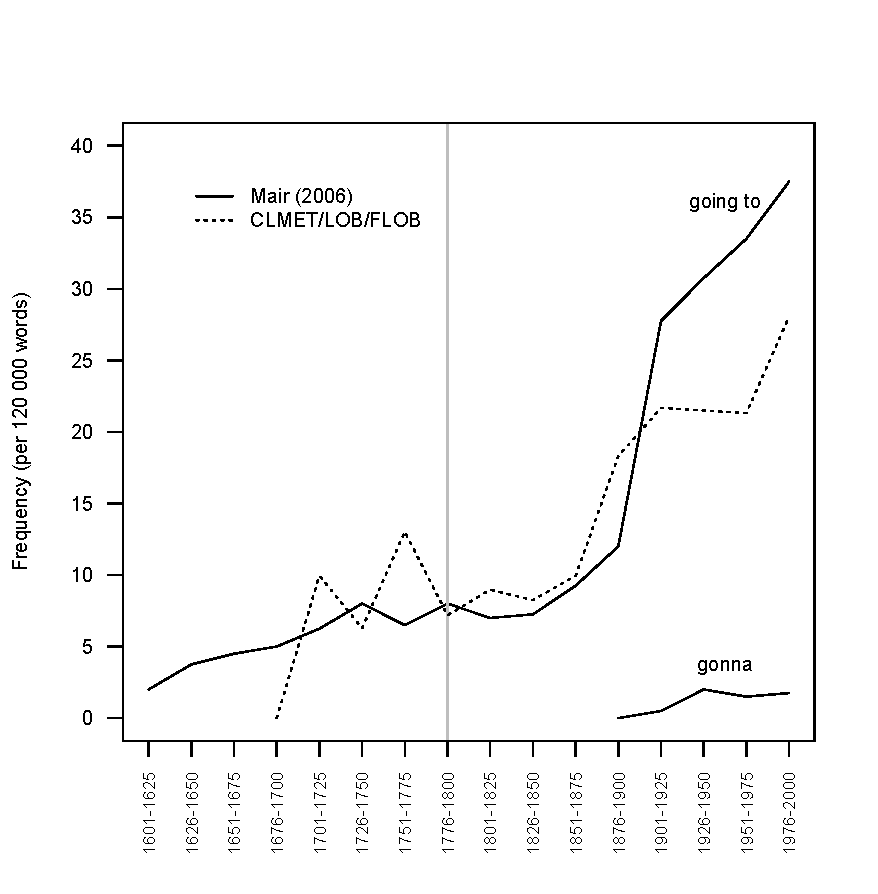
\includegraphics[width=.8\textwidth,keepaspectratio]{figures/goingtogrammaticalization}
\end{figure}

\begin{table}[!htbp]
\caption{Discourse frequency of \textit{going to}}
\label{tab:corpusgoingto}
\begin{tabular}[t]{c S[table-format=2] S[table-format=7] S l}
\lsptoprule
\multicolumn{1}{l}{\makecell[b]{Period \\ starting}} & \multicolumn{1}{l}{\makecell[b]{Raw \\ Freq.}} & \multicolumn{1}{l}{\makecell[b]{No. of \\ words}} & \multicolumn{1}{l}{\makecell[b]{Freq. p. \\ 120t words}} & \multicolumn{1}{l}{\makecell[b]{Data \\ Source}} \\
\midrule
1701 & 14 & 168799 & 9.95 & CLMET \\
1726 & 242 & 4623107 & 6.28 & CLMET \\
1751 & 591 & 5446006 & 13.02 & CLMET \\
1776 & 258 & 4308242 & 7.19 & CLMET \\
1801 & 231 & 3087842 & 8.98 & CLMET \\
1826 & 552 & 8024490 & 8.25 & CLMET \\
1851 & 442 & 5335906 & 9.94 & CLMET \\
1876 & 816 & 5349213 & 18.31 & CLMET \\
1901 & 722 & 3997155 & 21.68 & CLMET \\
1926 &  &  & 21.5 & (Extrapolated) \\
1951 & 180 & 1012985 & 21.32312 & LOB \\
1976 & 236 & 1009304 & 28.05894 & FLOB \\
\lspbottomrule
\end{tabular}
\end{table}

The grey line in Figure \ref{fig:mairgoingto} shows Mair's conservative estimate for the point at which the construction was firmly established as a way to express future tense). As the results from the OED citations and from the corpora show, there was only a small rise in frequency during the time that the construction became established, but a substantial jump in frequency afterwards. Interestingly, around the time of that jump, we also find the first documented instances of the contracted form \textit{gonna} (from Mair's data -- the contracted form is not frequent enough in the corpora used here to be shown). These results suggest, that semantic reanalysis is the first step in grammaticalization, followed by a rise in discourse frequency accompanied by phonological reduction.

This case study demonstrates that very large collections of citations can indeed be used as a corpus, as long as we are investigating phenomena that are likely to occur in citations collected to illustrate other phenomena: The results are very similar to those we get from well-constructed linguistic corpora. The case study also demonstrates the importance of corpora in diachronic research, a field of study which, as mentioned in Chapter \ref{ch:needforcorpus} has always relied on citations drawn from authentic texts, but which can profit from querying large collections of such texts and quantifying the results.

\subsection{Grammar and cultural analysis}
\label{sec:grammarandculturalanalysis}

Like words, grammatical structures usually represent themselves in corpus linguistic studies -- they are either investigated as part of a description of the syntactic behavior of lexical items or they are investigated in their own right in order to learn something about their semantic, formal or functional restrictions. However, like words, they can also be used as representatives of some aspect of the speech community's culture, specifically, a particular culturally defined scenario. To take a simple example: if we want to know what kinds of things are transferred between people in a given culture, we may look at the theme arguments of ditransitive constructions in a large corpus; we may look for collocates in the verb and theme positions of the ditransitive if we want to know \textit{how} particular things are transferred, cf. \citet{ludeling_corpora_2009}). In this way, grammatical structures can become diagnostics of culture, Again, care must be taken to ensure that the link between a grammatical structure and a putative scenario is plausible.

\subsubsection{Case study: He said, she said}
\label{sec:hesaidshesaid}

In a paper on the medial representation of men and women, \citet{caldas-coulthard_discourse_1993} finds that men are quoted vastly more frequently than women in the COBUILD corpus (cf. also Chapter \ref{ch:morphology}). She also notes in passing that the verbs of communication used to introduce or attribute the quotes differ -- both men's and women's speech is introduced using general verbs of communication, such as \textit{say} or \textit{tell} but with respect to more descriptive verbs, there are differences: ``Men \textit{shout} and \textit{groan}, while women (and children) \textit{scream } and \textit{yell}'' \citep[204]{caldas-coulthard_discourse_1993}.

The construction [QUOTE + Subj + V] is a perfect example of a diagnostic for a cultural frame: it is routinely used (in written language) to describe a speech event. Crucially, the verb slot offers an opportunity to introduce additional information (such as the manner of speaking, as in the examples of manner verbs verbs just mentioned (that often contain evaluations), but also the type of speech act being performed (\textit{ask}, \textit{order}), etc.). It is also easy to find even in an untagged corpus, since it includes (by definition) a passage of direct speech surrounded by quotation marks, a subject that is, in an overwhelming number of cases, a pronoun, and a verb (or verb group) -- typically in that order. In a written corpus, we can thus query the sequence $\langle$  \texttt{[word="{''}"] [pos="pronoun"] [pos="verb"]} $\rangle$ to find the majority of examples of the construction. In order to study differences in the representation of men and women, we can query the pronouns \textit{he} and \textit{she} separately to obtain representative samples of male and female speech act events without any annotation.

\begin{table}[!htbp]
\caption{Verbal collexemes of [QUOTE + Pron + V] (BNC)}
\label{tab:quotecollexemes}
\resizebox{\textwidth}{!}{%
\begin{tabular}[t]{l *{2}{S[table-format=4]} *{2}{S[table-format=8]} S}
\lsptoprule
\multicolumn{1}{c}{\makecell[tc]{\textvv{Verb}}} & \multicolumn{1}{c}{\makecell[tc]{Frequency with \\ \textvv{male subjects}}} & \multicolumn{1}{c}{\makecell[tc]{Frequency with \\  \textvv{female subjects}}} & \multicolumn{1}{c}{\makecell[tc]{Other words w. \\ \textvv{male subjects}}} & \multicolumn{1}{c}{\makecell[tc]{Other words w. \\ \textvv{female subjects}}} & \multicolumn{1}{c}{\makecell[tc]{G\textsuperscript{2}}} \\
\midrule
\multicolumn{6}{l}{Most strongly associated with \textvv{male subjects}} \\
\midrule
\textit{say} & 19301 & 11710 & 34916 & 26180 & 221.113740025537 \\
\textit{growl} & 158 & 5 & 54059 & 37885 & 131.833639357989 \\
\textit{drawl} & 172 & 10 & 54045 & 37880 & 122.790669077291 \\
\textit{write} & 239 & 56 & 53978 & 37834 & 66.2703036146206 \\
\textit{grate} & 80 & 4 & 54137 & 37886 & 59.7784278533784 \\
\textit{grin} & 301 & 89 & 53916 & 37801 & 58.4376336066056 \\
\textit{add} & 1526 & 771 & 52691 & 37119 & 57.0358747668258 \\
\textit{rasp} & 78 & 7 & 54139 & 37883 & 46.7825983195404 \\
\textit{continue} & 368 & 140 & 53849 & 37750 & 40.8160058329648 \\
\textit{snarl} & 82 & 13 & 54135 & 37877 & 34.1922679841907 \\
\textit{roar} & 54 & 5 & 54163 & 37885 & 31.88983015266 \\
\textit{chuckle} & 113 & 28 & 54104 & 37862 & 28.9961524072897 \\
\textit{murmur} & 633 & 311 & 53584 & 37579 & 27.1042800738047 \\
\textit{comment} & 117 & 34 & 54100 & 37856 & 23.3699450627582 \\
\textit{shout} & 349 & 155 & 53868 & 37735 & 23.3398935606577 \\
\textit{gesture} & 93 & 24 & 54124 & 37866 & 22.4960822128815 \\
\textit{grunt} & 51 & 8 & 54166 & 37882 & 21.4475135121844 \\
\textit{boom} & 26 & 1 & 54191 & 37889 & 20.7846724511177 \\
\textit{wink} & 34 & 3 & 54183 & 37887 & 20.549582166759 \\
\textit{claim} & 69 & 16 & 54148 & 37874 & 19.3533927260091 \\
\midrule
\multicolumn{6}{l}{Most strongly associated with \textvv{female subjects}} \\
\midrule
\textit{whisper} & 393 & 666 & 53824 & 37224 & 205.213509030231 \\
\textit{cry} & 216 & 395 & 54001 & 37495 & 137.792857031815 \\
\textit{feel} & 94 & 206 & 54123 & 37684 & 92.8582736796259 \\
\textit{manage} & 32 & 116 & 54185 & 37774 & 85.5960328992645 \\
\textit{snap} & 174 & 275 & 54043 & 37615 & 73.8061205295948 \\
\textit{retort} & 75 & 155 & 54142 & 37735 & 64.5876647672653 \\
\textit{protest} & 60 & 136 & 54157 & 37754 & 63.8828166553974 \\
\textit{giggle} & 13 & 61 & 54204 & 37829 & 53.4026088768348 \\
\textit{try} & 85 & 152 & 54132 & 37738 & 50.9082148546456 \\
\textit{ask} & 2136 & 1860 & 52081 & 36030 & 49.9523882508786 \\
\textit{flush} & 5 & 41 & 54212 & 37849 & 46.5313347509488 \\
\textit{wail} & 8 & 46 & 54209 & 37844 & 44.9207452054127 \\
\textit{swallow} & 24 & 71 & 54193 & 37819 & 44.2276081076112 \\
\textit{gasp} & 69 & 125 & 54148 & 37765 & 42.7478681479244 \\
\textit{exclaim} & 137 & 196 & 54080 & 37694 & 42.4370037780204 \\
\textit{force} & 9 & 45 & 54208 & 37845 & 40.8456344052239 \\
\textit{flare} & 1 & 27 & 54216 & 37863 & 40.4086421411062 \\
\textit{hear} & 82 & 130 & 54135 & 37760 & 35.0120478684469 \\
\textit{sob} & 13 & 45 & 54204 & 37845 & 32.0195724567643 \\
\textit{blush} & 3 & 27 & 54214 & 37863 & 31.6506392273931 \\
\lspbottomrule
\end{tabular}}
\end{table}
% query: BNC; [word="(?|\")"] [word="(he|she)"%c][pos=".*VV.*"]; count Last by hw on match[1]..match[2]

This design can be applied deductively, if we have hypotheses about the gender-specific usage of particular (sets of) verbs, or inductively, if we simply calculate the association strength of all verbs to one pronoun as compared to the other. In either case we have two nominal variables, \textsc{Subject of Quoted Speech}, with the variables \textsc{male} (\textit{he}) and \textsc{female} (\textit{she}), and \textsc{Speech Activity Verb} with all occurring verbs as its values. Table \ref{tab:quotecollexemes} shows the results of an inductive application of the design to the BNC.

There is a clear difference that corroborates Caldas-Coulthard's casual observation: the top ten verbs of communication associated with men contain five verbs conveying a rough, unpleasant and/or aggressive manner of speaking (\textit{growl}, \textit{grate}, \textit{rasp}, \textit{snarl}, \textit{roar}), while those for women only include one (\textit{snap}, related to irritability rather than outright aggression). Interestingly, two very general communication verbs \textit{say} and \textit{write}, are also typical for men's reported speech. Women's speech is introduced by verbs conveying weakness or communicative subordination (\textit{whisper}, \textit{cry}, \textit{manage}, \textit{protest}, \textit{wail} and \textit{deny}).

\subsection{Grammar and counterexamples}
\label{sec:grammarandcounterexamples}

While this book focuses on quantitative designs, non-quantitative designs are possible within the general framework adopted. Chapter \ref{ch:scientificmethod} included a discussion of counterexamples and their place in a scientific framework for corpus linguistics. Let us conclude this chapter with a case study making use of them.

\subsubsection{Case study: \textit{To}- vs. \textit{that}-complements}
\label{sec:tovsthatcomplements}

A good case study for English that is based largely on counterexamples is \citet{rohdenburg_is_2003}, who looks at a number of claims made about the semantics of infinitival complements as compared to \textit{that}-clauses. He takes claims made by other authors based on their intuition and treats them like Popperian hypotheses, searching the BNC for counterexamples. He mentions more or less informal impressions about frequencies, but only to clarify that the counterexamples are not just isolated occurrences that could be explained away.

For example, he takes the well-known claim that with verbs of knowing, infinitival complements present knowledge as subjective/personal, while \textit{that-}clauses present knowledge as objective/impersonal/public. This is supposed to explain acceptability judgments like the following (\citet[45--46]{corum_be_1973}, \citet[50, 136]{wierzbicka_semantics_1988}):

\begin{exe}
\ex
\begin{xlist} 
\label{ex:findtobe}
\ex He found her to be intelligent.
\ex[*]{I bet that ifyou look in the files, you'll find her to be Mexican.}
\ex I bet that if you look in the files, you'll find that she is Mexican.
\end{xlist}
\end{exe}

The crucial counterexample here would be one like (\ref{ex:findtobe}b), with an infinitival complement that expresses knowledge that is ``public'' rather than ``personal/experiential''; also of interest would be examples with \textit{that}-clauses that express personal/experiential knowledge. The corresponding queries are easy enough to define:

\begin{exe}
\ex
\begin{xlist} 
\label{ex:findtobequery}
\ex \begin{minipage}[t]{0.85\textwidth} \raggedright \texttt{[word="(find|\allowbreak finds|\allowbreak finding|\allowbreak found)"\%c]} \texttt{[word="(me|\allowbreak you|\allowbreak him|\allowbreak her|\allowbreak it|\allowbreak us|\allowbreak them)"\%c]} \texttt{[word="to"\%c]} \texttt{[word="be"\%c]} \end{minipage}
\ex \begin{minipage}[t]{0.85\textwidth} \raggedright \texttt{[word="(find|\allowbreak finds|\allowbreak finding|\allowbreak found)"\%c]} \texttt{[word="that"\%c]} \texttt{[word="(I|\allowbreak you|\allowbreak he|\allowbreak she|\allowbreak it|\allowbreak we|\allowbreak they)"\%c]} \texttt{[word="(is|\allowbreak are|\allowbreak was|\allowbreak were)"\%c]} \end{minipage}
\end{xlist}
\end{exe}

This query follows the specific example in (\ref{ex:findtobe}b) very narrowly, we could of course define a broader one that would capture, for example, proper names and noun phrases in addition to pronouns, but remember that we are looking for counterexamples -- if we can find these with a query following the structure of supposedly non-acceptable sentences very closely, they will be all the more convincing.

The BNC contains not just one, but many counterexamples. Here are some examples with \textit{that}-complements expressing subjective, personal knowledge:

\begin{exe}
\ex
\begin{xlist} 
\label{ex:findthatsubjective}
\ex Erika was surprised to find that she was beginning to like Bach (BNC A7A)
\ex $[$A$]$che of loneliness apart, I found that I was stimulated by the challenge of finding my way about this great and beautiful city. (BNC AMC)
\end{xlist}
\end{exe}

And here are some with \textit{to}-complements expressing objective, impersonal knowledge:

\begin{exe}
\ex
\begin{xlist} 
\label{ex:findtobefact}
\ex Li and her coworkers have been able to locate these sequence variations ... in the three-dimensional structure of the toxin, and found them to be concentrated in the $\beta$ sheets of domain II. (BNC ALV)
\ex The visiting party, who were the first and last ever to get a good look at the crater of Perboewetan, found it to be about \num{1000} metres in diameter and about fifty metres deep (BNC ASR)
\end{xlist}
\end{exe}

These counterexamples (and others not cited here) in fact give us a new hypothesis as to what the specific semantic contribution of the \textit{to}-complement may be: if used to refer to objective knowledge, it overwhelmingly refers to situations where this objective knowledge was not previously known to the participants of the situation described. In fact, if we extend our search for counterexamples beyond the BNC to the world-wide web, we find examples that are even more parallel to (\ref{ex:findtobe}b), such as (\ref{ex:findtobenationality}), all produced by native speakers of English:

\begin{exe}
\ex
\begin{xlist} 
\label{ex:findtobenationality}
\ex Afterwards found that French had stopped ship and found her to be German masquerading as Greek. (www.hmsneptune.com)
\ex I was able to trace back my Grandfathers name ... to Scotland and then into Sussex and Surrey, England. Very exciting! Reason being is because we were told that the ancestors were Irish and we found them to be Scottish! (www.gettheeblowdryer.com)
\ex Eishaus -- This place is an Erlangen institution, should you ever get to meet the owner you'll find him to be American, he runs this wonderful ice cream shop as his summer job away from his `proper' job in the states. (theerlangenexpat.wordpress.com)
\end{xlist}
\end{exe}

Again, what is different in these examples from the (supposedly unacceptable) example (\ref{ex:findtobe}b) is that the knowledge in question is new (and surprising) to the participants of the situation. This observation could now be used as the basis for a new hypothesis concerning the difference between the two constructions, but even if it is not or if this hypothesis turned out to be false, the counterexamples clearly disprove the claim by Wierzbicka and others concerning the subjective/objective distinction (\citet{rohdenburg_is_2003} actually goes on to propose an information-structural account of the difference between the \textit{to-} and the \textit{that}-complement).

This case study was intended to show how counterexamples may play a role in disproving hypotheses based on introspection and constructed examples (see \citet{meurers_use_2005} and \citet{meurers_corpora_2009} as good examples for the theoretically informed search for counterexamples).

